\documentclass[14pt]{report}

\usepackage{Packages}
\usepackage{Commands}

\begin{document}

\maketitle

\tableofcontents

\if 0

\chapter{2 курс}
\section{Введение}

Модель случайных блужданий без самопересечений (далее - СБС) - одна из наиболее широко изученных моделей из класса линейных полимеров. 
Более того, она является одной из простейших моделей для изучения критического поведения - так, в случае когда модель усложнена наличием взаимодействия между ближайшими узлами цепочки, её фазовый переход оказывается зафиксирован между состояниями её растворителя, и при термическом равновесии системы полученная полимерная цепочка будет схлопнутой в условиях сильного растворителя или вытянутой в слабом растворителе.
Трикритичность данного перехода была описана в работе \cite{Gennes1979}.

Влияние близких связей было широко рассмотрено среди класса моделей магнитного полимера, взаимодействие между узлами которых стало ещё более сложным:
каждый узел обладает спином, а сила взаимодействия между ближайшими узлами стала отдельным параметром. 
Её название - модель Изинга на случайном блуждании без самопересечений.
В работе \cite{Garel1999} был рассмотрен случай, когда она так же обладает переменным внешним полем, и все заключения о её магнитных свойствах были оценены в сравнении с моделью среднего поля.
В то же время влияние геометрических свойств модели на магнитные не до конца ясно и их изучение в некоторых случаях требует статистического подхода.

В предыдущей работе \cite{faizullina2021critical} было определено, что фазовый переход двумерной модели Изинга на CБС
имеет непрерывный характер. 
В этой работе мы продолжаем изучать геометрические свойства данной модели и сравнивать их с её родительскими моделями или модификациями, такими как классическая модель Изинга на регулярной решётке, опредёленная в работе \cite{selke2006critical}, и взаимодействующее случайное блуждание без самопересечений в соответствующих критических областях. 
Мы предполагаем, что модели с похожими геометрическими свойствами будут так же иметь схожесть в магнитных, что мы рассмотрим при сравнении кумулянтов биндера в области $\theta$-перехода моделей при равных значениях асферичности.
Также могут быть интересны для рассмотрения решётки, на которых исследуются конформации модели, как параметр задающий закон, по которому определяется близость узлов и следовательно - существование тех или иных связей между ними в цепочке. 
Данное направление было начато в частном случае среди концов случайных блужданий без самопересечений на квадратной решётке в работе \cite{owczarek2008scaling}. 
В нашей работе мы рассмотрим эти результаты с долей узлов с фиксированным количество соседей на квадратной решётке, как обобщение на внутренние узлы цепочки, а так же рассмотрим поведение данного геометрического свойства среди разных решёток в пределе бесконечной длины цепочки.  

\section{Модели и методы}
В рамках данной работы определяется несколько моделей: первой будет модель Изинга на случайном блужданий без самопересечений (далее - Ising-ISAW). Энергия системы конформации $u$ (последовательности точек на решётке, на которых размещёна цепочка) фиксированной длины N с последовательностью спинов в узлах s, принимающих значение $+1$ или $-1$, рассчитывается как сумма взаимодействий между ближайшими узлами цепочки:

\begin{equation}
E(s,u) = -J \sum_{\la i, j \ra} s_i s_j,\ \ \ \ i,j \in u, |u|=N
\end{equation}
Статическая сумма модели берётся по всем возможным последовательностяv ${s}$ и конформациям $u$:

\begin{equation}
Z = \sum_s \sum_u \exp{(\frac{-E}{kT})}
\end{equation}

где $T$ — температура, $k$ — постоянная Больцмана. Без потери общности можно считать $kT = 1$, тем самым оставляя J самостоятелньым параметром модели.
В первой части работы модель Ising-ISAW рассматривается только на квадратной решётке, где соседями узла можно считать мономеры, расположенные сверху, снизу, слева и справа от него.

Под "родительскими" к Ising-ISAW моделями определим следующие две: с одной стороны, взаимодействующая составляющая модели берётся из классических моделей Изинга - в частности, мы будем рассматривать классическую модель Изинга на регулярной прямоугольной решётке (далее - прямоугольный Изинг), определеную так же в работе \cite{selke2006critical}.
В ней узлы со спинами заполняют всю решётку со стороной $L=N_x$ и отношением сторон $r=\frac{N_y}{N_x}$. Длина стороны считается как количество узлов решётки в одном ряде. 
Решётка может иметь как периодический граничные условия - когда узлы на противоположных краях решётки считаются соседними - так 
Тогда энергия системы с последовательностью спинов $s$, рассчитывается как сумма взаимодействий между ближайшими узлами по всей решётке:

\begin{equation}
E(L, r, \{s\}) = -J \sum_{\la i, j \ra} s_i s_j,\ \ \ \ i,j = (x_i, u_i), (x_j, y_j) \in [1..L] \times [1..L*r]
\end{equation}

Статическая сумма модели берётся только возможным последовательностяv ${s}$:

\begin{equation}
Z = \sum_s \exp{(\frac{-E}{kT})}
\end{equation}

В качестве сравниваемого между моделями магнитного свойства определим кумулянт Биндера (или критический кумулянт):

\begin{equation}
\label{eq:Cumulant}
U_{4} = 1 - \frac{\la m^{4} \ra}{3 (m^{2})^{2}}
\end{equation}

где $\la m^{2} \ra$  - средний квадрат удельной намагниченности, $\la m^{4} \ra$ - средная удельная намагниченность в четвертой степени. 

С другой стороны, определелим модель взаимодействующего блуждания без самопересечений (далее - ISAW) на квадратной решётке из работы \cite{caracciolo2011geometrical}.
В отличие от Ising-ISAW, узлы конформации не имеют спинов, и энергия модели рассчитывается как сумма связей переменной силы J между узлами:

\begin{equation}
E(\{u\}) = \sum_{\la i, j \ra} 1,\ \ \ i,j \in u, |u|=N
\end{equation}

\begin{equation}
Z = \sum_s \exp{(- \beta E(\{s\}))}
\end{equation}

В рамках работы \cite{caracciolo2011geometrical} исследовалось поведение геометрических свойств в критической области - в частности, асферичности конформации, показателя отличия системы узлов от круга.
Для этого определим показатели формы системы, такие как тензор вращения системы - матрица корреляции координат системы из N точек $w_i = (w_{i,\alpha}, w_{i,\beta})$:

\begin{equation}\label{eq:Ten_G1}
    Q_{N,\alpha\beta} = \frac{1}{N+1} \sum^{N}_{i=0}(w_{i,\alpha} - w_{c, \alpha})(w_{i,\beta} - w_{c, \beta})
\end{equation}

где $w_{c,\alpha} - \alpha$ -я координата вектора центра масс. В случае, если начало координат расположено в центре масс (следовательно, сумма векторов точек блуждания = 0), формула $\alpha\beta-$элемента тензора упрощается и численно равна второму моменту координаты (если $\alpha = \beta$), или до среднего произведения разных координат по всем точкам блуждания.

\begin{align}\label{eq:Ten_G_C}
    Q_{N,\alpha\beta} = &\frac{1}{(N+1)} \sum_{i=0}^{N} w_{i, \alpha} w_{i, \beta} \\
    \sum^{N}_{i=0}w_{i} &= 0
\end{align}

Собственные значения $q_1, q_2$ полученного тензора вращения можно интерпретировать как квадраты длин полуосей эллипса вращения системы.
Их отношение для системы длины $N$ равна:

\begin{equation}
r = \sqrt{\frac{\la q_1 \ra_N}{\la q_2 \ra_N}}
\end{equation}

Так же эти значения используются для расчёта ещё одного показателя формы -
средней асферичности:

\begin{equation}
\label{eq:Asphericity}
    \mathcal{A} = \left\langle \frac{(q_{1} - q_{2})^{2}}{(q_{1} + q_{2})^{2}} \right\rangle_{N}
\end{equation}

Модификации исследуемой системы Ising-ISAW имеют изменения в выбранной решётке - то есть, законов, по кото
: в работе





\section{Средняя намагнинченность случая h = 0}

По предыдущим расчетам мы знаем формулу ср. намагниченности, с самого начала считая J = 0. С одной стороны, по определению среднего:

\begin{equation}\label{MeanMagnJ01}
    \la\sigma\ra = \frac{1}{ZN} \int S\ e^{-\beta H},\  H = -h\sum_{j=1}^{N}\sigma_{j} = -h S
\end{equation}

где S - сумма всех моментов в цепи. С другой стороны: 

\begin{equation}\label{MeanMagnJ02}
    \frac{1}{ZN} \int S\ e^{-\beta H} = \frac{\partial Log[Z_{J = 0}]}{\partial h} \frac{1}{\beta N} = \frac{1}{Z \beta N}  \dzdh
\end{equation}

В этом случае Z берется сразу при условии (J = 0), её гамильтонианом для N спинов при периодичном и открытом гран. условии будет \eqref{Hh}, а статсуммой будет формула (30.8) при (30.10) из учебника Свендсена \cite{swendsen2020introduction}:

\begin{gather}
    \label{Zh0} Z_{j = 0} = (2\cosh{\bh})^N \\
    \label{Z'hh0} \dzdh_{j = 0} = \beta N 2^{N}(\cosh{\bh})^{N-1}\sinh{\bh}
\end{gather}

Следовательно, при подстановке в \eqref{MeanMagnJ02}, получим:

\begin{equation}\label{MeanMagnJ0Final}
    \la\sigma\ra = \frac{1}{Z \beta N}  \dzdh = \tanh{(\bh)}  
\end{equation}

Применим эту операцию для статсуммы общего случая.
Для упрощения задачи будем рассматривать случай h = 0.

\subsection{Периодичные гран. условия}

Перед этим для простоты найдём производные всех составляющих статсумм:

\begin{equation}\label{Q'h}
    (Q)^{'}_{h} = \frac{1}{2\sqrt{e^{2\bj} \cosh{(\bh)}^{2} - 2 \sinh{(2\bj)}}}  \left( e^{2\bj}2\cosh{(\bh)} \sinh{(\bh)}  \beta\right)
\end{equation}

и при (h = 0) = 0

Тогда:

\begin{equation}\label{lpm'h}
    (\lpm)^{'}_{h} = e^{\bj}  \sinh{(\bh)} \beta \pm (Q)^{'}_{h}
\end{equation}

и при (h = 0) так же = 0

Таким образом: 

\begin{equation}\label{MeanMagnH0PBC}
    \la\sigma\pbc\ra = \frac{1}{Z  \beta  N}  \frac{\partial Z}{\partial h} = \frac{1}{Z  \beta  N}  \left( N  \lambda^{N-1}_{+}(\lambda_{+})^{'}_{h} +   \lambda^{N-1}_{-}(\lambda_{-})^{'}_{h}\right) = 0
\end{equation}

\subsection{Открытые гран. условия}

Найдём дополнительные значения составляющих $Z\obc$

$Q_{h = 0} = e^{-\bj}$

Также найдём значения $\lambda_{\pm}$ при h = 0
\begin{equation}\label{lpmH0}
    \lambda_{\pm (h=0)} = e^{\bj} \pm \sqrt{e^{2\bj} - \left( e^{2\bj} - e^{-2\bj} \right)} = e^{\bj} \pm e^{-\bj}
\end{equation}

Тогда $ \lambda_{+ (h = 0)} = 2\cosh{\bj} $ и $ \lambda_{- (h = 0)} = 2\sinh{\bj} $

Рассмотрим производную $Z\obc$ по h, учитывая дифференцирование произведения и все полученные ранее результаты (\eqref{Q'h}, \eqref{lpm'h}, \eqref{lpmH0})

\begin{multline}\label{Zobc'h}
    \frac{\partial Z}{\partial h} = \lp^{N-1}(\frac{e^{\bj}2\sinh{\bh}\ \cosh{\bh}\ \beta Q - (Q)^{'}_{h}e^{\bj}\sinh{\bh}^{2}}{Q^{2}} - \frac{(Q)^{'}_{h}}{e^{\bj}Q^{2}} + \beta\sinh{\bh}) - 
    \\
    - \lm^{N-1}(\frac{e^{\bj}2\sinh{\bh}\ \cosh{\bh}\ \beta Q - (Q)^{'}_{h}e^{\bj}\sinh{\bh}^{2}}{Q^{2}} - \frac{(Q)^{'}_{h}}{e^{\bj}Q^{2}} - \beta\sinh{\bh}) =_{h=0} 0
\end{multline} 

Следовательно, $ \la\sigma\obc\ra = 0 $


\subsection{Магнитная воприимчивость}

Мы выяснили, что средняя намагниченность одномерной цепи при любом гран. условии равна нулю. Рассмотрим в таком случае магнитную восприимчивость $ X = \frac{\partial \langle m \rangle}{\partial h}$

Учитывая формулу намагниченности \eqref{MeanMagnJ01} и то, что первая производная статсуммы \eqref{Zobc'h} равна нулю:

\[ X = (\frac{1}{Z \beta} \dzdb)^{'}_{h} = \frac{1}{\beta} (\dzdb (- \frac{1}{Z^{2}} \dzdb) + \frac{1}{Z} \frac{\partial^{2} Z}{\partial h^{2}}) = \frac{1}{Z \beta} \frac{\partial^{2} Z}{\partial h^{2}}\]

После расчётов, представленных в .nb файле (раздел 21.10.2020 (поиск X)) получим:

\[ X = \frac{\beta}{2} (2Ne^{2\bj} - e^{4\bj} + 1) + \frac{\beta}{2} \tanh^{N-1}\bj (e^{4\bj} - 2 e^{2\bj} + 1)\]

Подстановка $ T = 0, \infty$ приведёт к одинаковому результату и обратной зависимости от T, что говорит о парамагнетических свойствах одномерной модели Изинга.
\section{Средняя энергия}

Чтобы удостовериться в правильности полученной формулы для статсуммы общего случая открытого гран. условия \eqref{Zobc}, проверим её на предельных условиях (h = 0, J = 0), поскольку они были рассмотрены в учебнике \cite{Swen}.

Нам известна формула средней энергии:
\begin{equation}\label{MeanE}
    \la U \ra = -\frac{\partial Log[Z]}{\partial \beta} = \frac{1}{Z} \dzdb
\end{equation}

Предварительно будет нелишним найти значения составных частей формулы и их производных по $\beta$

\[ \lambda_{\pm}^{'} = e^{\bj}J\cosh{\bh} + e^{\bj}\sinh{\bh}\ h \pm \]
\[\pm \frac{1}{Q}  (e^{\dbj}J\cosh{\bh} + e^{\dbj}\cosh{\bh}\ \sinh{\bh}\ h - \cosh{\dbj}\ 2J) \] 

В виду большого числа различных значений, составим таблицу всех составных значений в формуле.
\begin{table}[h!]\label{derLTab}
    \centering
    \begin{tabular}{c c c c c c c}
         & $\lp$ & $(\lp)^{'}_{\beta}$ & $\lm$ & $(\lm)^{'}_{\beta}$ & $Q$ & $(Q)^{'}_{\beta}$  \\ \\
        h = 0 & $2\cosh{\bj}$ & $2J\sinh{\bj}$ & $2\sinh{\bj}$ & $2J\cosh{\bj}$ & $e^{-\bj}$ & $-J e^{-\bj}$ \\
        J = 0 & $2\cosh{\bh}$ & $2h\sinh{\bh}$ & $0$ & $0$ & $\cosh{\bh}$ & $h\sinh{\bh}$\\
    \end{tabular}
    \caption{Производные составных значений статсумм}
\end{table}



\subsection{Проверка случая J = 0}

Теперь можно перейти к проверке по предельным случаям.
\[ Z\obc(h = 0) = 2^{N-1}\cosh{\bj}^{N-1} (0 + 1 + 1) - 2^{N-1}\sinh{\bj}^{N-1} (0 + 1 - 1) = 2^{N}\cosh{\bj}^{N-1}\]

\[ Z\obc(J = 0) = 2^{N-1}\cosh{\bh}^{N-1} (\frac{(\sinh{\bh})^{2} + 1}{\cosh{\bh}} +\cosh{\bh}) = \]
\[=2^{N-1}\cosh{\bh}^{N-1} (\frac{(\cosh{\bh})^{2}}{\cosh{\bh}} +\cosh{\bh}) = \]

\[= 2^{N}\cosh{\bh}^{N}\]

Как и ожидалось, статсуммы совпали с расчетами учебника \cite{Swen}, что говорит о правильности формулы. Чтобы сильнее убедиться в этом, найдём формулы средней энергии. 

Для J = 0 заранее учтём, что правое слагаемое формулы статсуммы и её производной обнулится:
\[\dzdb = \lp^{N-1}(\frac{e^{\bj}\sinh{\bh}((J\sinh{\bh} + 2h\cosh{\bh})Q - (Q)^{'}_{\beta}\sinh{\bh})}{Q^{2}} - \]
\[ - \frac{J Q + (Q)^{'}_{\beta}}{e^{\bj} Q^{2}} + h\sinh{\bh}) + \lp^{N-2} (\lp)^{'}_{\beta}(N-1)(\frac{e^{\bj} \sinh{\bh}^2}{Q} + \frac{1}{e^{\bj}Q} + \cosh{\bh})\]
При подстановке J=0 мы получим $2^{N}(\cosh{\bh})^{N-1}N\sinh{\bh}$

И в конечном счёте формула средней энергии системы при J=0: 

\[\langle U_{J = 0} \rangle = - \frac{1}{Z} \dzdb = - N h\tanh{\bh}\]

Даннная формула полностью совпадает с расчётами в учебнике \cite{Swen}, что говорит о правильности формулы для статсуммы обобщенного случая.

\subsection{Случай h = 0}

Из проделанных ранее расчётов для средней энергии системы при случае h = 0, используя соответствующую статсумму, мы получили следующую формулу:
\[ \langle U_{h = 0} \rangle = - J(N - 1)\tanh{\bj} \]
Попробуем вывести ту же формулу через статсумму общего случая.

Начнём со статсуммы:
\[ Z\obc(h=0) = \lp^{N-1}(0 + 1 + 1) - \lm^{N-1}(0 + 1 - 1) = 2^{N}(\cosh{\bj})^{N-1}\]
Поскольку формула производной статсуммы увеличится в два раза из-за ненулевых $\lm$ и $(\lm)^{'}_{\beta}$ рассмотрим их сомножители, заранее учитывая их отличие лишь в знаке правого $\cosh{\bh}$. Назовём их $A_{+}$ и $A_{-}$

Так, при подстановке в производную как $А_{+}$, так и $A_{-}$  h=0 получим ноль. А при подстановке h=0 в сами сомножители, получим:
\[A_{+(h=0)} = 2\]
\[A_{-(h=0)} = 0\]
Таким образом, наша формула $\dzdb_{h=0}$ сократилась в 4 раза и равна:
\[ \dzdb_{h=0} = (N-1)\lp^{N-2}(\lp)^{'}_{\beta}2 = J(N-1)2^{N}(\cosh{\bj})^{N-1}\sinh{\bj}\]

Итоговая формула средней энергии будет:
\[ \langle U_{h=0} \rangle = - \frac{1}{Z} \dzdb = - J (N - 1) \tanh{\bj}\]

\subsection{Сравнение средней энергии моделей с периодичным и открытым гран. условиями}

Найдём формулу средней энергии для случая с периодичным гран. условием для h = 0. Воспользовавшись формулой \eqref{Zpbc} для нахождения средней энергии через \eqref{MeanE} и таблицей производных, получим:

\begin{align*}
    \la E_{PBC (h = 0)} \ra = \frac{1}{Z\pbc(h = 0)}\left(N\lp^{N-1}(\lp)\prpb + N\lm^{N-1}(\lm)\prpb \right) = \\
    = JN2^{N}\sinh{\bj}\ \cosh{\bj} \frac{(\cosh{\bj})^{N-2} + (\sinh{\bj})^{N-2}}{(\cosh{\bj})^{N} + (\sinh{\bj})^{N}} = \\
    = JN2^{N} \tanh{\bj} \frac{1 + (\tanh{\bj})^{N-2}}{1 + (\tanh{\bj})^{N}} \approx \footnotemark JN2^{N} \tanh{\bj}
\end{align*}

\footnotetext{\begin{align*}
        \frac{1+(\tanh{x})^{N-2}}{1+(\tanh{x})^{N}} = \frac{1+x^{N}(\dfrac{1}{x^{2}} + (\dfrac{2}{3} - \dfrac{n}{3}) + O(x))}{1+x^{N}(1 - \dfrac{nx^{2}}{3} + O(x^{3}))} \approx 1 & ,\ x \to 0,\ \ \ \  1, x \to \infty
    \end{align*}}
\section{Теплоёмкость на спин при h = 0}
Теперь, поскольку наша формула статсуммы $Z\obc$ (для крайних случаев) и её производная (для средних наблюдаемых) полностью верна, проверим правильность статсуммы до второй производной по $\beta$ для нахождения темплоёмкости на спин С в случае нулевого поля.

\subsection{Открытое гран. условие}

Из учебника данная формула выглядит следующим образом:

\begin{equation}\label{HeatCapH0}
c = \frac{1}{N} \frac{\partial U}{\partial T} = - \frac{1}{N k_{B} T^{2}} \frac{\partial U}{\partial \beta} \approx k_{B} \beta^{2} J^{2} (sech \bj)^{2}    
\end{equation}

Предыдущие вычисления уже показали правильность формулы средней энергии, однако для более полной проверки выразим U через статсумму, и следовательно:

\[ -\frac{1}{N k_{B} T^{2}} \frac{\partial U}{\partial \beta} = - k_{B} \beta^{2} \frac{1}{N} \frac{\partial}{\partial \beta} (- \frac{1}{Z} \dzdb) = k_{B} \beta^{2} \frac{1}{N} (- \frac{1}{Z^{2}} (\dzdb)^{2} + \frac{1}{Z} \frac{\partial^{2} Z}{\partial \beta^{2}}) \]

Теперь для определения второйй производной статсуммы перейдём к той же замене, как в конце предыдущего раздела:

\[ Z\obc = \lp^{N-1} A_{+} - \lm^{N-1} A_{-} \]
\[ (Z\obc)\prpb = (N-1) \lp^{N-2} (\lp)\prpb A_{+} + \lp^{N-1} (A_{+})\prpb - (N-1) \lm^{N-2} (\lm)\prpb A_{-} - \lm^{N-1} (A_{-})\prpb \]

Т.к. мы знаем, что первые производные $(A_{\pm})\prpb = 0$ и $A_{-} = 0, A_{+} = 2$, то половина второй производной (вследствие производной произведения) обнулится. Будет лучше заранее найти значения вторых производных А и $\lpm$ при h = 0.

\[ (A_{\pm})\vprpb =_{h=0} 0 \]
\[ (\lpm)\vprpb =_{h=0} J^{2}(e^{\bj} \pm e^{-\bj}) \]

Таким образом, единственным необнулённым слагаемым второй производной будет первое и:
\[ Z\obc = 2\lp^{N-1} \]
\[ (Z\obc)\prpb = 2(N-1) \lp^{N-2} (\lp)\prpb\]
\[ (Z\obc)\vprpb = 2(N-1)((N-2)\lp^{N-3}(\lp)\prpb ^{2} + \lp^{N-2}(\lp)\vprpb) \]

Раскрыв все $\lp$ и подставив в формулу теплоёмкости на спин, получим:
\[ c = k_{B} \beta^{2} (1 - \frac{1}{N}) (- (N-1) (\frac{(\lp)\prpb}{\lp})^{2} + (N-2) (\frac{(\lp)\prpb}{\lp})^{2} + \frac{(\lp)\vprpb}{\lp}) =\]
\[ = k_{B} \beta^{2} J^{2} (1 - \frac{1}{N}) (1 - (\frac{\sinh{\bj}}{\cosh{\bj}})^{2}) \approx k_{B} \beta^{2} J^{2} (sech \bj)^{2} \]

Формулы полностью совпали.

\subsection{Периодическое гран. условие}

Формула теплоёмкости на спин для данного условия отсутствует в учебнике, поэтому сравнить полученный результат с первоисточником не получится и к вычислениям данной формулы требуется особое внимание.

Начнём с формулы статсуммы:
\[ Z\pbc = \lambda_{+}
 ^{N} + \lambda _{-} ^{N} = \lp^{N}(1 + (\frac{\lp}{\lm})^{N}) =_{h=0} 2^{N} (\cosh{\bj})^{N} (1 + (\tanh{\bj})^{N}) \]
 
 \[ (Z\pbc)\prpb = N(\lp^{N-1} (\lp)\prpb + \lm^{N-1} (\lm)\prpb) = J N 2^{N} (\cosh{\bj})^{N-1} \sinh{\bj} (1 + (\tanh{\bj})^{N-2}) \]
 
 \[ (Z\pbc)\vprpb = N (\lp^{N-1} (\lp)\vprpb) + (N-1)\lp^{N-2} (\lp)\prpb^{2} + \lm^{N-1} (\lm)\vprpb) + (N-1)\lm^{N-2} (\lm)\prpb^{2}) = \]
 
 \[ = 2^{N} N J^{2} (\cosh{\bj})^{N} (1 + (N-1)(\tanh{\bj})^{2} + (N-1)(\tanh{\bj})^{N-2} + \tanh{\bj})\]
 
Прошлые расчёты показали, что формула теплоёмкости на спин выражается через статсумму как:

\[ c = \frac{k_{B} \beta^{2}}{N} (- \frac{1}{Z^{2}} (\dzdb)^{2} + \frac{1}{Z} \frac{\partial^{2} Z}{\partial \beta^{2}}) \]

В таком случае, при подстановке статсуммы и производных, мы получим:

\[ c = k_{B} \beta^{2} J^{2} \left(1 + (N-1) \tanh^{2}\bj (\frac{1 + \tanh^{N-4}\bj}{1 + \tanh^{N}\bj}) - N \tanh^{2}\bj (\frac{1 + \tanh^{N-2}\bj}{1 + \tanh^{N}\bj})^{2}\right) \]

В случае термодинамического предела, все дроби вида $ \frac{1 + \tanh}{1 + \tanh}$ стремятся к единице (есть небольшое отклонение, которое при увеличении N смещается вправо и одновременно уменьшается. Тогда в итоге:

\[ c = k_{B} \beta^{2} J^{2} sech^{2} \bj \]
\section{Свободная энергия}
Учитывая предыдущие вычисления, будет удобно проверить формулу другой величины - свободной энергии дл 
я случая h = 0. Для этого слегка преобразуем нашу статсумму:
\[ Z\obc = \lp^{N-1}A_{+}(1 - (\frac{\lm}{\lp})^{N-1}(\frac{A_{-}}{A_{+}}) \]

где \[ A_{+} = \frac{e^{\bj} \sinh{\bh}^2}{Q} + \frac{1}{e^{\bj}Q} +  \cosh{\bh}\]
\[ A_{-} = \frac{e^{\bj} \sinh{\bh}^2}{Q} + \frac{1}{e^{\bj}Q} -  \cosh{\bh}\]

Тогда свободная энергия для случая h=0 будет равна:
\[ F_{h=0} = k_{B}T\ln{Z} =  k_{B}(N-1)\ln{\lp} + k_{B}T\ln{A+} + k_{B}T\ln{(1 - (\frac{\lm}{\lp})^{N-1}(\frac{A_{-}}{A_{+}}))}\]

Ранее мы узнали все преобразования при h = 0: $A_{+} = 2, A_{-} = 0$, следовательно:
\[ F_{h=0} = k_{B}T(N-1)\ln{(2\cosh{\bj})} + k_{B}T\ln{2}\]

Результаты снова совпали с формулой из учебника \cite{Swen}.

Тогда руководствуясь предыдущими расчётами для случая J=0, свободная энергия для данного случая (зная, что $\lp = 2\cosh{\bh}, \lm = 0, A_{+} = 2\cosh{\bh}$) будет равна:
\[ F_{J=0} = k_{B}T N \ln{(2\cosh{\bh})}\]
\section{Разница между открытым и периодичным случаем}

Будем рассматривать разность между различными энергетическими величинами при разных случаев.

\subsection{Средняя энергия системы (равное число спинов)}


Найдём разность средней энергии открытого и периодичного случая:

\begin{equation}\label{DiffMeanE1}
    \la U\obc \ra - \la U\obc \ra = -\frac{\partial Log[Z\obc]}{\partial \beta} + \frac{\partial Log[Z\pbc]}{\partial \beta} = -\frac{\partial Log[\frac{Z\obc}{Z\pbc}]}{\partial \beta}
\end{equation}

\[ \frac{Z\obc}{Z\pbc} = \frac{A_{+}\left( 1 + (\frac{\lambda_{-}}{\lambda_{+}})^{N - 1}  \frac{A_{-}}{A_{+}}\right)}{\lambda{+}(1 + (\frac{\lambda_{-}}{\lambda_{+}})^{N})} \]

\[ \apm = \frac{e^{\bj} \sinh{\bh}^2}{Q} + \frac{1}{e^{\bj}Q} \pm \cosh{\bh} \]

Учитывая что мы рассматриваем системы при $N \rightarrow \infty$,
все скобки вида $ Log[ 1 + (<1)^{N} ] \approx (<1)^{N} $ 

Тогда

\begin{equation}\label{diffMeanE2}
     \la U\obc \ra - \la U\pbc \ra =  -\frac{\partial ( Log[\frac{Z\obc}{Z\pbc}])}{\partial \beta} = -\frac{\partial}{\partial \beta} \left(Log[\frac{A_{+}}{\lambda{+}}] + (\frac{\lambda_{-}}{\lambda_{+}})^{N - 1}(\frac{A_{-}}{A_{+}} - \frac{\lm}{\lp}) + o((\frac{\lambda_{-}}{\lambda_{+}})^{N-1})\right)
\end{equation}

Перед тем, как продолжить расчёты, стоит заранее найти производные отношений $\frac{\lm}{\lm}$ и $\frac{\am}{\ap}$. 

Тогда производная их частного будет выглядеть как:

\[ (\frac{\lm}{\lp})\prpb = \frac{(\lm)\prpb\lp-\lm(\lp)\prpb}{\lp^{2}}\]

Все значения для крайних случаев можно легко взять из нашей таблицы.

\[ h = 0: \frac{J}{\cosh^{2}\bj} \]

\[ J = 0: 0 \]

Теперь перейдём к $\apm$. Поскольку они имеют одинаковые слагаемые, отличающиеся по знаку, то для упрощения можно представить их как:

\[ \apm = A_{0} \pm \cosh{\bh} \]

Тогда при дифференцировании частного половина слагаемых в числителе сократится, а другая сложится:

\[ (\frac{\am}{\ap})\prpb = \frac{(\am)\prpb\ap-\am(\ap)\prpb}{\ap^{2}} = \frac{(A_{0}' - h\sinh{\bh})(A_{0} + \cosh{\bh}) - (A_{0} - \cosh{\bh})(A_{0}'+ h\sinh{\bh})}{\ap^{2}} = \]

\[ = 2\frac{A_{0}'\cosh{\bh} - A_{0}h\sinh{\bh}}{\ap^{2}}\]

Формулу $A_{0}'$ и значения $\apm$ для предельных значении можно взять из расчётов производной статсуммы и средней энергии. При предельных случаях производная частного $\am$ и $\ap$ обращается в ноль.

Теперь вернёмся к формуле \eqref{diffMeanE2} и продифференцируем всю скобку по $\beta$

\begin{equation}\label{diffMeanE3}
    \la U\obc \ra - \la U\pbc \ra = -\frac{(\ap)\prpb}{\ap} + \frac{(\lp)\prpb}{\lp} + N(\frac{\lm}{\lp})^{N-1}(\frac{\lm}{\lp})\prpb - (N-1)(\frac{\lm}{\lp})^{N-2}(\frac{\lm}{\lp})\prpb(\frac{\am}{\ap}) - (\frac{\lm}{\lp})^{N-1}(\frac{\am}{\ap})\prpb
\end{equation}

Рассмотрим все значения и значения производных по $\beta$ $ \lambda_{+}$ и $A_{+}$ при h = 0 и J = 0 из таблицы.

Путём подстановки в полученную формулу производной \eqref{diffMeanE3}, получим:

\[ h = 0:\ \ J + JN\frac{(\tanh{\bj})^{N-1}}{(\cosh{\bj})^{2}} \approx_{N\to\infty} J\ \ \footnotemark\]

\[J = 0: 0\]

\footnotetext{
\begin{align*}
    \frac{(\tanh{x})^{N-1}}{(\cosh{x})^{2}} &= x^{N-1} + o(x^{N}) \approx 0,\ x\to 0 \\
    &= \frac{\to1}{\to\infty} \approx 0,\ x\to\infty
\end{align*}}

\subsection{Средняя энергия системы (равное число рёбер)}

Рассмотрим теперь случай с равным числом ребёр - он достигается при сравнении моделей с периодическим гран. условием с N спинами и с открытым гран. условием с N+1 спинами, тогда формула \eqref{diffMeanE2} станет:

\begin{equation}\label{diffMeanER1}
    \la U\obc \ra - \la U\pbc \ra = -\frac{\partial}{\partial \beta}\left(Log[\ap]+(\frac{\lm}{\lp})^{N}(\frac{\am}{\ap} - 1) + o((\frac{\lambda_{-}}{\lambda_{+}})^{N})\right)    
\end{equation}

Все дополнительные расчёты производных мы сделали в предыдущем подразделе, поэтому перейдём к изменённой формуле, аналогичной \eqref{diffMeanE3}, и затем сразу к предельным случаям:

\begin{equation}\label{diffMeanER2}
    \la U\obc \ra - \la U\pbc \ra = -\frac{(\ap)\prpb}{\ap} - N(\frac{\lm}{\lp})^{N-1}(\frac{\lm}{\lp})\prpb (\frac{\am}{\ap} - 1) - (\frac{\lm}{\lp})^{N}(\frac{\am}{\ap})\prpb
\end{equation}

\[ h = 0: JN\frac{(\tanh{\bj})^{N-1}}{(\cosh{\bj})^{2}} \approx_{N\to\infty} 0 \]

\[ J = 0: -h\tanh{\bh}\]

\subsection{Теплоёмкость системы (равное число рёбер)}

Формулу для теплоёмкости системы возьмём из \eqref{HeatCapH0} без деления на N:

\begin{equation}\label{eq:HeatCap}
c=\frac{\partial U}{\partial T} = -\frac{1}{k_{B}T^{2}}\frac{\partial U}{\partial \beta} = \frac{1}{k_{B}T^{2}}\frac{\partial^{2} Log[Z]}{\partial \beta^{2}}
\end{equation}

Так как мы рассматриваем случай равных ребёр, то как и в прошлый раз, возьмём систему из N спинов для модели с периодическим гран. условием и систему из N+1 спинов для модели с открытым гран. условием - таким образом мы получим вторую производную знакомого нам выражения из формулы \eqref{diffMeanER1}: 

\begin{equation}\label{diffHeatCapER1}
  c\obc^{N+1} - c\pbc^{N} = \frac{1}{k_{B}T^{2}} \frac{\partial^{2}}{\partial \beta^{2}} Log[\frac{Z\obc}{Z\pbc}] = \frac{1}{k_{B}T^{2}} \frac{\partial^{2}}{\partial \beta^{2}} \left(Log[\ap]+(\frac{\lm}{\lp})^{N}(\frac{\am}{\ap} - 1) + o((\frac{\lambda_{-}}{\lambda_{+}})^{N})\right)  
\end{equation}

Рассмотрим первые два слагаемых выражения в скобках по отдельности, чтобы не запутаться в расчётах:

\begin{equation*}
    (Log[\ap])\vprpb = \frac{(\ap)\vprpb}{\ap} - (\frac{(\ap)\prpb}{\ap})^{2}
\end{equation*}

\[ ((\frac{\lm}{\lp})^{N}(\frac{\am}{\ap} - 1))\vprpb = \]
\[ = N(N-1)(\frac{\lm}{\lp})^{N-2}(\frac{\lm}{\lp})^{'2}(\frac{\am}{\ap} - 1) + N(\frac{\lm}{\lp})^{N-1}(\frac{\lm}{\lp})\vprpb(\frac{\am}{\ap} - 1) + 2N(\frac{\lm}{\lp})^{N-1}(\frac{\lm}{\lp})\prpb(\frac{\am}{\ap})\prpb + (\frac{\lm}{\lp})^{N}(\frac{\am}{\ap})\vprpb \]

Все вспомогательные расчёты для предльных случаев были сделаны в Wolfram Mathematica (Проект2.pdf, Теплоёмкость)\cite{Git}, поэтому пропустим этот шаг и перейдём к итоговым выражениям:

\[ h = 0:\ -N(N-1)J^{2}\frac{(\tanh{\bj})^{N-2}}{(\cosh{\bj})^{2}} \]
\[ J = 0:\ 0\]

\subsection{Квадрат намагниченности системы (равное число рёбер)}

Формула среднего квадрата намагниченности во многом схожа с формулой теплоёмкости при предельных случаях. С одной стороны, по определению средней наблюдаемой величины, квадрат намагничесности представима в виде:

\begin{equation}
    \la M^{2} \ra = \frac{1}{Z} \sum_{\{\sigma\}} M^{2} e^{-\beta H},
\end{equation}
где H - гамильтониан системы \eqref{eq:Ham}.

С другой стороны:

\begin{equation}
    \frac{1}{Z} \sum_{\{\sigma\}} M^{2} e^{-\beta H} = \frac{1}{\beta^{2}}(\frac{\partial^{2} \log{Z}}{\partial h^{2}} + (\frac{\partial \log{Z}}{\partial h})^{2}) = \la M^{2} \ra
\end{equation}

Правое слагаемое в скобке является квадратом средней намагниченности, который при предельных случаях равна нулю, поэтому нам достаточно только левого. Это значит, что в формуле разности будет то же самое выражение под знаком дифференцирования, что и в формулах \eqref{diffMeanER1} и \eqref{diffHeatCapER1}. Опять же, мы берём N+1 спин для открытого условия, и N для периодического. Тогда:

\begin{equation}\label{eq:diffSqMagnER1}
    \la M^{2}\obc \ra - \la M^{2}\pbc \ra = \frac{1}{\beta^{2}} \frac{\partial^{2}}{\partial h^{2}} Log[\frac{Z\obc}{Z\pbc}] = \frac{1}{\beta^{2}} \frac{\partial^{2}}{\partial h^{2}} \left(Log[\ap]+(\frac{\lm}{\lp})^{N}(\frac{\am}{\ap} - 1) + o((\frac{\lambda_{-}}{\lambda_{+}})^{N})\right)  
\end{equation}

Воспользуемся расчётами Wolfram Mathematica (Проект2.pdf, Квадрат намагниченности), и получим: 

\[ h = 0:\ \frac{1}{2}(2e^{2\bj}-e^{4\bj}+1)+2N(\tanh{\bj})^{N}-2e^{2\bj}(\sinh{\bj})^{2}(\tanh{\bj})^{n}\]
\[ J = 0:\ 1-(\tanh{\bj})^{2}\]
\section{Сравнение решения одномерной модели Изинга с расчётами Монте-Карло}

Для сравнения значений наблюдаемых из решения для одномерной модели Изинга и расчётов методом Монте-Карло были расмотрены значения средней энергии на спин, удельной теплоёмкости, и среднего квадрата намагниченности на спин с формулами соответственно: 

\begin{align*}
    \la U \ra &= \bj (1 - \frac{1}{N}) \tanh{\bj} \\
    c &= (\bj)^{2} (1 - \frac{1}{N}) (sech \bj )^{2} \\
    \la m^{2} \ra &= (\frac{e^{2\bj} - 1}{N})^{2} (\tanh{\bj})^{N-1} + 2 \frac{e^{2\bj}}{N} + \frac{1 - e^{4\bj}}{n^2}
\end{align*}

(Расчёт последней формулы описан в Проект7.1.pdf\cite{web:ProjectMagnetRepos})

Были проведены расчёты для длин от 250 до 10000, сейчас полученные данные находятся в обработке.
\section{Поведение модели Изинга вблизи крит. температуры}

Критическая область - одна из сложнейших областей для изучения поведения любой термодинамической модели, как для теоретическим, так и экспериментальным способом. В частности, есть предположение, что модель Изинга вблизи крит. температуры показывает схожесть в поведении с фазовым переходом жидкой/парообразной системы в области тройной точки, что даёт интересный повод для изучения данной области и расчётов критических экспонент с помощью симуляций Монте-Карло.

Определим приведённую температуру t как "расстояние" от критической температуры:

\begin{equation} \label{eq:redTemp}
    t = \frac{T - T_{C}}{T_{C}}
\end{equation}

T - текущая температура модели, $T_{C}$ - критическая температура. Тогда корреляционная длина при термодинамическом пределе (системе бесконечной длины) в критической области будет:

\begin{equation}\label{eq:CorLen}
    \xi \sim \mid t \mid ^{-\upsilon} 
\end{equation}
где $\upsilon$ - критическая экспонента

Также мы можем определить другие экспоненты - к примеру, в нормальной модели Изинга определяются экспоненты $\gamma$, $\alpha$ и $\beta$ для магнитной восприимчивости, темпоёмкости и намагниченности соответственно:

\begin{equation}
    \chi \sim \mid t \mid ^{-\gamma}
\end{equation}

\begin{equation}
    c \sim \mid t \mid ^{-\alpha}
\end{equation}

\begin{equation}
    m \sim \mid t \mid ^{-\beta}
\end{equation}

Рассмотрим случай квадрата намагниченности:

\begin{equation}
    m^{2} \sim \mid t \mid ^{-2\beta}
\end{equation}

Воспользовавшись \eqref{eq:CorLen}, избавимся от t:

\begin{equation}
    m^{2} \sim \xi ^{2\beta/\upsilon}
\end{equation}

учитывая поведение корреляционной длины в конечноразмерных системах (книга "Monte Carlo Methods in Statistical Physics", график 4.1 и стр. 232-233)\cite{NewBar}, мы можем представить функцию квадрата намагниченности в виде:

\begin{equation}\label{eq:m2_1}
    m^{2} = \xi ^{-2\beta/\upsilon} m_{02}(L/\xi)
\end{equation}

Где L - размер системы (для квадратной решётки кол-во спинов = L * L)

$m_{02}$ обладает следующими свойствами:

\begin{align*}
    m_{02}(x) = C,\ \ x >> 1 \\
    m_{02}(x) \sim x^{-2\beta/\upsilon},\ \ x \rightarrow 0
\end{align*}

Так как \eqref{eq:m2_1} содержит неизвестную нам корреляционную длину, преобразуем её с новой безразмерной функцией:

\begin{equation}
    \Tilde{m}_{02}(x) = x^{-2\beta} m_{02}(x^{\upsilon})
\end{equation}

Тогда получим:

\begin{equation}\label{eq:m2_2}
    m^{2} = L^{-2\beta/\upsilon} \Tilde{m}_{02}(L^{1/\upsilon}|t|)
\end{equation}

\subsection{Расчёты крит. экспонент при наблюдении коллапса данных}
Для того, чтобы найти крит. экспоненты $\beta$ и $\upsilon$, а также крит. температуру модели, достаточно определить, при каких их значениях графики шкалирующих функций $\Tilde{m}_{02}$ для разных размеров L системы сливаются к как можно более однородному графику. Для этого значение шкал. функции расчитывается из \eqref{eq:m2_2}:

\begin{equation}\label{eq:m02}
    \Tilde{m}_{02} = L^{2\beta/\upsilon} m_{L}^{2}(t)
\end{equation}

В случае квадрата намагниченности наилучший коллапс данных наблюдался при:

\begin{align*}
    T_{C} = 1.1976 \\
    \beta = 0.125 \\
    \upsilon = 1.01
\end{align*}

\begin{figure}[!h]
    \centering
    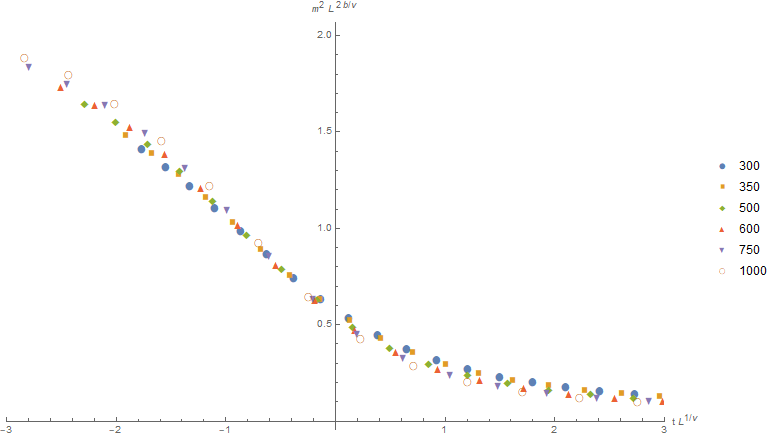
\includegraphics[width=100mm]{Sections/Images/DatColMagn2_3.png}
    \label{fig:DatColM2_3}
\end{figure}

\subsection{Определение погрешностей измерений экспонент}

Разумеется, поскольку мы не можем численно определить качество коллапса данных, а лишь визуально определить при каких значениях он будет лучше, необходимо задать погрешность - область значений критических экспонент и температур, при которых качество коллапса данных наблюдаемой величины при измерении "на глаз" не меняется.

Таким образом, мы уточняем возможные критические значения для сравнения с расчётов в других источниках, для определения модели по её поведению.

\begin{figure}[h]
\begin{minipage}[h]{0.5\linewidth}
\center{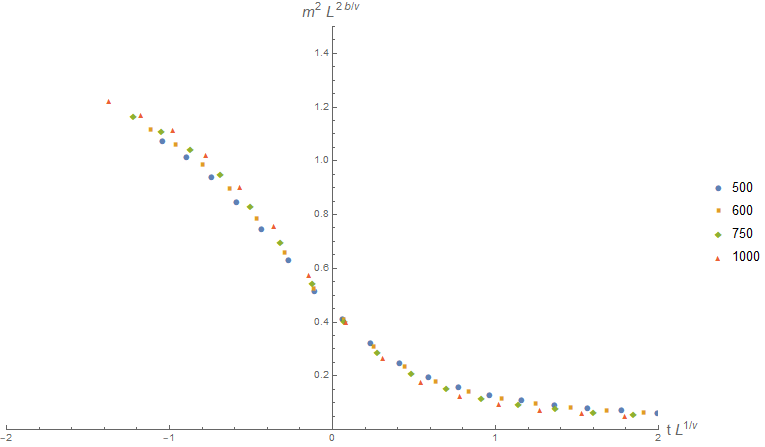
\includegraphics[width=0.9\linewidth]{Sections/Images/DataCollLowExp.png} \\ $\beta = 0.04,\ \nu = 0.8$}
\end{minipage}
\hfill
\begin{minipage}[h]{0.5\linewidth}
\center{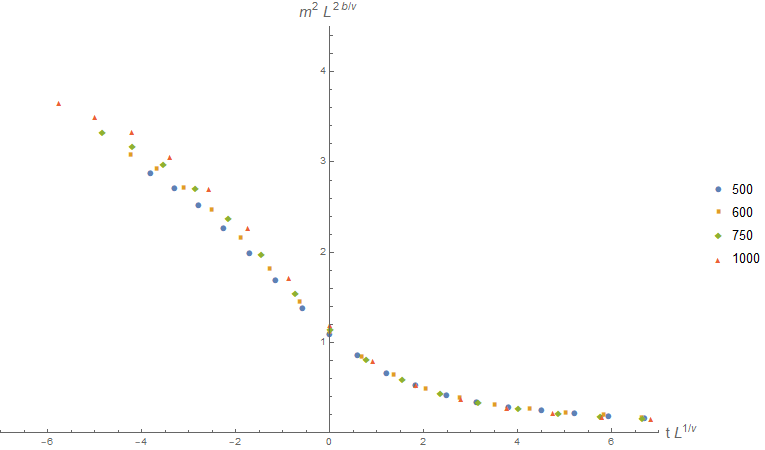
\includegraphics[width=0.9\linewidth]{Sections/Images/DataCollHighExp.png} \\ $\beta = 0.3,\ \nu = 1.2$}
\end{minipage}
\caption{Погрешность критических экспонент и их влияние на коллапс данных}
\label{ris:image1}
\end{figure}

Из графиков видно, что несмотря на колоссальное отличие от расчитанных из литературы\cite{NewBar} значений, качество коллапса данных для квадрата намагниченности едва отличается между графиками - отличие заключается лишь в их масштабе - что говорит о серьёзной погрешности данного метода для расчёта критических показателей модели.
\section{Модель прямоугольного Изинга}

В данном разделе мы будем рассматривать зависимость наблюдаемых модели Изинга от формы решетки: в частности, от отношения сторон в прямоугольной решётке

\subsection{Расчёт критических кумулянтов для модели прямоугольного Изинга}

Кумулянт Биндера для модели Изинга в критической точке расчитывается по формуле:
\begin{equation}
\label{eq:Cumulant}
U_{4} = 1 - \frac{\la m^{4} \ra}{3 * (m^{2})^{2}}
\end{equation}

где $\la m^{2} \ra$ - средний квадрат удельной намагниченности, $\la m^{4} \ra$ - средная удельная намагниченность в четвертой степени. 

Для сравнения значения кумулянтов модели прямоугольного Изинга с разными размерами, но одинаковым отношением сторон (так же Aspect Ratio или r), так, что число спинов составляет L * rL были проведены симуляции модели на основе алгоритма из проектной работы Сорокина Никиты \cite{Schro} и Камиллы Файзулиной \cite{SAW} - для этого были взяты длины 50, 100, 200 и 400 и отношения сторон 1/4, 1/2, 3/4 при $2 * 10^{6}$ итераций.

\begin{figure}[!h]
    \centering
    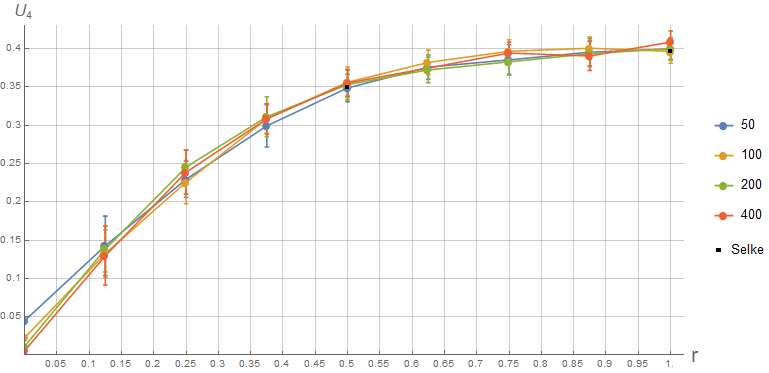
\includegraphics[width=100mm]{Sections/Images/CumulantOBC.png}
    \caption{График зависимости значения кумулянта Биндера в крит. точке от Aspect Ratio при открытых гран. условиях}
    \label{fig:CumulOBC}
\end{figure}

\begin{figure}[!h]
    \centering
    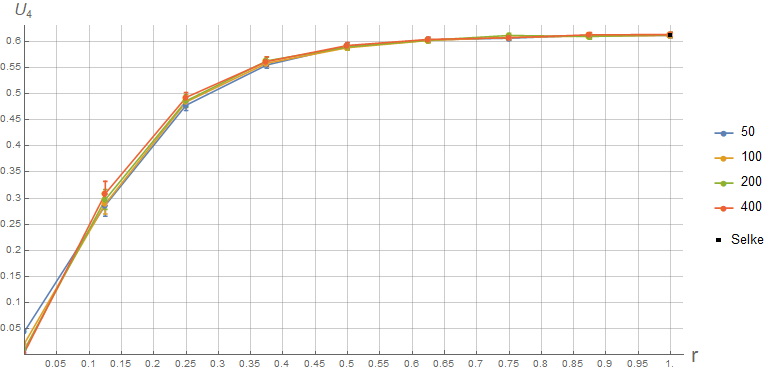
\includegraphics[width=100mm]{Sections/Images/CumulantPBC.png}
    \caption{График зависимости значения кумулянта Биндера в крит. точке от Aspect Ratio при периодических гран. условиях}
    \label{fig:CumulPBC}
\end{figure}

Крайние левые точки в отметке нуля являются расчётами для модели одномерного Изинга (где длина цепочки равна соответствующей стороне в двумерном изинге). Так, в случае открытых гран. условий (рис. \ref{fig:CumulOBC}) и периодических (рис. \ref{fig:CumulPBC}) значения кумулянта стремится к нулю с увеличением длины цепочки(см. Проект6.pdf\cite{Git}).
Черными точками отмечены значения критического кумулянта из работы Уолтера Сельке - 0.396 ± 0.002 для квадратной модели и 0.349 ± 0.002 для прямоугольной с отношением сторон r = 1/2 при открытых гран. условий. Для периодического случая квадратной модели критический кумулянт равен 0.61069\cite{Selke}.

Эти же значения отмечены в графиках \ref{fig:CumulOBCL} и \ref{fig:CumulPBCL} зависимости крит. кумулянта от обратной длины стороны как крайние левые (в нуле - так обозначен случай термодинамического предела).

\begin{figure}[!h]
    \centering
    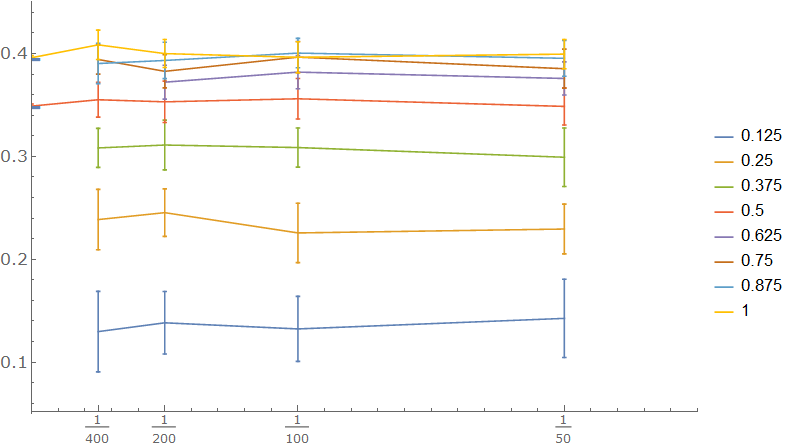
\includegraphics[width=100mm]{Sections/Images/CumulantOBCL.png}
    \caption{График зависимости значения кумулянта Биндера в крит. точке от обратной длины стороны при открытых гран. условиях}
    \label{fig:CumulOBCL}
\end{figure}

\begin{figure}[!h]
    \centering
    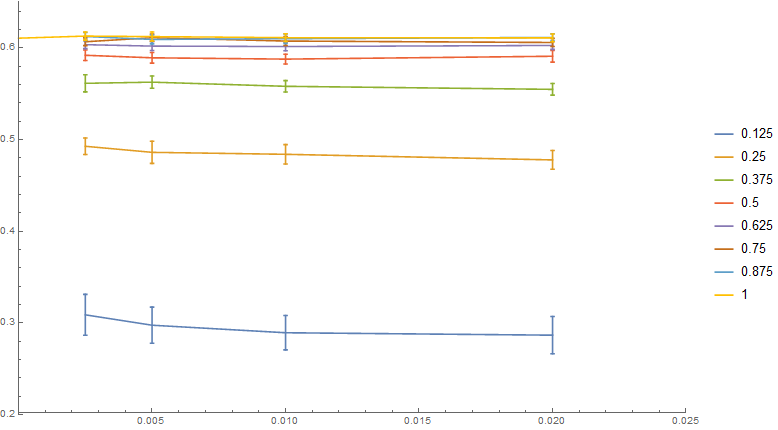
\includegraphics[width=100mm]{Sections/Images/CumulantPBCL.png}
    \caption{График зависимости значения кумулянта Биндера в крит. точке от обратной длины стороны при периодических гран. условиях}
    \label{fig:CumulPBCL}
\end{figure}

Учитывая погрешность в расчётах симуляций, зависимость от обратной длины прямоугольника 1/L не наблюдается.

\subsection{Сравнение модели Изинга и модели взаимодействующих непересекающихся блужданий}

Здесь мы рассмотрим основные понятия в модели взаимодействующих блужданий (Self-Avoiding Walks, SAWs), связанные с их формой и сравним их с прямоугольной моделью в тех же условиях. 

Важнейшим параметром в описании полученной симуляциями Монте-Карло блуждания является радиус инерции, численно равный среднему квадратическому расстоянию частиц от положения среднего арифметического центра модели (сумма $w_{k}$ в скобке)\cite{Pelissetto}:

\begin{equation}\label{eq:Rg}
    R^{2}_{g} = \frac{1}{N+1} \sum^{N}_{i=0}\left(w_{i} - \frac{1}{N+1}\sum^{N}_{k=0}w_{k}\right)^2 = \frac{1}{2(N+1)^{2}}\sum^{N}_{i,j=0}(w_{i} - w_{j})^{2}
\end{equation}

Так же для описания формы модели применяется тензор вращения относительно центра масс - матрица, $\alpha\beta-$й элемент которой расчитывается по формуле (4) из статьи\cite{Janke_G} :

\begin{equation}\label{eq:Ten_G1}
    Q_{N,\alpha\beta} = \frac{1}{N+1} \sum^{N}_{i=0}(w_{i,\alpha} - w_{c, \alpha})(w_{i,\beta} - w_{c, \beta})
\end{equation}
где $w_{c,\alpha} - \alpha$ -я координата вектора центра масс. В случае, если начало координат расположено в центре масс (следовательно, сумма векторов точек блуждания = 0), формула $\alpha\beta-$элемента тензора упрощается и численно равна второму моменту координаты (если $\alpha = \beta$), или до среднего произведения разных координат по всем точкам блуждания.


\begin{align}\label{eq:Ten_G_C}
    Q_{N,\alpha\beta} = &\frac{1}{(N+1)} \sum_{i=0}^{N} w_{i, \alpha} w_{i, \beta} \\
    \sum^{N}_{i=0}w_{i} &= 0
\end{align}

Рассмотрим формулу \eqref{eq:Ten_G1}. Так так $w{c}$ - центра масс блуждания, то:

\begin{equation}
    w_{c} = \frac{1}{N+1} \sum_{k=0}^{N} w_{k}
\end{equation}

Так же можно представить i-й вектор блуждания как:

\begin{equation}
    w_{i} = \frac{1}{N+1} \sum_{k=0}^{N} w_{i}
\end{equation}

Это позволит нам вытащить из скобок N+1 и избавиться от неизвестного $w_{c}$

\begin{align*}
    Q_{N,\alpha\beta} = \frac{1}{(N+1)^{3}} \sum^{N}_{i=0}(\sum^{N}_{k=0}(w_{i,\alpha} - w_{k, \alpha}))(\sum^{N}_{l=0}(w_{i,\beta} - w_{l, \beta})) = \\
    = \frac{1}{(N+1)^{3}} \sum^{N}_{i=0} \sum^{N}_{k,l=0}(w_{i,\alpha} - w_{k, \alpha})(w_{i,\beta} - w_{l, \beta}) = \\
    \frac{1}{(N+1)^{3}} \sum^{N}_{i=0} \sum^{N}_{k,l=0} (w_{i,\alpha} w_{i,\beta} - w_{i,\alpha} w_{l,\beta} - w_{k,\alpha} w_{i,\beta} + w_{k,\alpha} w_{l,\beta})
\end{align*}

Расскроем суммирование у учётов зависимостей индексов:

\begin{align*}
    Q_{N,\alpha\beta} = \frac{1}{(N+1)^{2}} (\sum^{N}_{i,k=0}(w_{i,\alpha} w_{i,\beta}) - \sum^{N}_{i,l=0}(w_{i,\alpha} w_{l,\beta}) - \sum^{N}_{i,k=0}(w_{k,\alpha} w_{i,\beta}) + \sum^{N}_{k,l=0}(w_{k,\alpha} w_{l,\beta})) = \\
    \frac{1}{(N+1)^{2}} \sum^{N}_{i,k=0}(w_{i,\alpha} w_{i,\beta} - w_{k,\alpha} w_{i,\beta}) = \frac{1}{2(N+1)^{2}} \sum^{N}_{i,k=0}(w_{i,\alpha} - w_{k, \alpha})(w_{i,\beta} - w_{k, \beta})
\end{align*}
т.к. кол-во произведений координат разных векторов и одинаковых меньше в два раза. Полученная формула:

\begin{equation}\label{eq:Ten_G2}
    Q_{N,\alpha\beta} \frac{1}{2(N+1)^{2}} \sum^{N}_{i,k=0}(w_{i,\alpha} - w_{k, \alpha})(w_{i,\beta} - w_{k, \beta})
\end{equation}

совпадает с формулой (4.1) из статьи о взаимодействующих блужданиях\cite{Pelissetto}, что значит что используемое ими понятие "тензора вращения" совпадает.

\subsection{Тензор инерции и тензор вращения}

Можно заметить некоторое сходство в расчётах недиагональных элементов тензора инерции J и тензора вращения из статей\cite{Pelissetto, Yanke_G}. Действительно, для системы из N материальных точек единичной массы тензор инерции в системе центра масс рассчитывается следующим образом:

\begin{equation}
    J = \left(
    \begin{array}{ccc}
        J_{xx} & J_{xy} & J_{xz}  \\
        J_{yx} & J_{yy} & J_{yz} \\
        J_{zx} & J_{zy} & J_{zz}
    \end{array} \right)
\end{equation}

\begin{align}
    J_{xy} &= J_{yx} = -\sum_{i=1}^{N} x_{i} y_{i} \\
    J_{yz} &= J_{zy} = -\sum_{i=1}^{N} y_{i} z_{i} \\
    J_{xz} &= J_{zx} = -\sum_{i=1}^{N} x_{i} z_{i} 
\end{align}

В тоже время, формулы диагональных элементов принципиально отличаются:

\begin{align}
    J_{xx} &= \sum_{i=1}^{N} y_{i}^{2} + z_{i}^{2} \\
    J_{yy} &= \sum_{i=1}^{N} x_{i}^{2} + z_{i}^{2} \\
    J_{zz} &= \sum_{i=1}^{N} x_{i}^{2} + y_{i}^{2}
\end{align}

Сравнивая с формулой элементов тензора вращения в системе центра масс \eqref{eq:Ten_G_C}, можно заметить, что недиагональные элементы тензоров отличаются знаком и усреднением в тензоре вращения. Диагональные же элементы "противоположны" друг другу:
в тензоре инерции они обозначают осевые моменты инерции (относительно $O\alpha$, и поэтому обозначенные моменты одной координатой ($J_{\alpha\alpha}$ используют сумму квадратов отличных от $\alpha$ координат.

Таким образом, элементы тензора вращения в системе центра масс в трехмерном простанстве можно представить как:

\begin{equation}
   Q_{\alpha\alpha} = \frac{1}{N}\sum^{N}_{i=1}w_{i,\alpha}^2 = \frac{1}{N} \left(\sum_{i=1}^{N}x_{i}^{2} + y_{i}^{2} + z_{i}^{2} - J_{\alpha\alpha}\right) = R^{2}_{g} - \frac{1}{N} J_{\alpha\alpha}  
\end{equation}

где $w_{i,\alpha}$ - $\alpha$-я координата радиус-вектора i-й материальной точки.

\begin{equation}
    Q_{\alpha\beta} = -\frac{1}{N} J_{\alpha\beta},\ \ \alpha \neq \beta
\end{equation}

Тогда матричный вид формулы тензора вращения через тензор инерции будет:

\begin{equation}
    Q = R_{g}^{2} * E - \frac{1}{N} J
\end{equation}
где E - это единичная матрица порядка, совпадающим с размерностью данной модели Dim.

Мы знаем, что симметричная матрица (какой являются и Q, и J) всегда диагонализируема, а базис из собственных векторов - ортогонален. Пусть S - матрица перехода в жорданов базис тензора инерции. Произведём переход в этот базис для тензора вращения:

\begin{equation*}
    S^{T}QS = S^{T} (R_{g}^{2} * E - \frac{1}{N} J) S = R^{2}_{g} * S^{T}ES-\frac{1}{N} * S^{T}JS
\end{equation*}

Матрица S - ортогональна, следовательно $S^{-1} = S^{T}$, поэтому:

\begin{equation}
    S^{T}QS = R^{2}_{g} * E - \frac{1}{N} * J_{D}
\end{equation}

где $J_{D}$ - диагонализированная матрица тензора инерции. Очевидно, что полученная в правой части матрица - диагональная. Следовательно, матрица в левой части так же получилась диагональной полсе перехода в новый базис и жорданов базис тензоров инерции и вращения одинаковы, пусть и с разными собственными значениями. Соответствующие собственные значения матриц в жордановом базисе будут равны:

\begin{align*}
    (S^{T}QS)_{ii} = Q_{D, ii} = R^{2}_{g} - \frac{1}{N}J_{ii},\ \ i=1..Dim
\end{align*}

Стоит подчеркнуть, что если жорданов базис составлен так, что собственные значения тензора инерции в матрице упорядочены по неубыванию, то в тензоре вращения собственные значения в матрице в этом базисе же будут упорядочены по невозрастанию.

\subsection{Показатели формы блуждания из тензора вращения}

Так как полученная матрица симметричная, то существует такой поворот, преобразующий её в диагональную (т.е., приводящий систему в Жорданов базис с собственными значениями по диагонали, и нулевыми недиагональными элементами), причём так, чтобы значения на диагонали были положительными и упорядоченными по невозрастанию.

В нашем двумерном случае, 

\begin{equation*}
    Q_{N} = \left(
    \begin{array}{cc}
      q_{1} & 0 \\
      0 & q_{2}
    \end{array} \right),\ 0 < q_{2} \leq q_{1}
\end{equation*}

Отметим так же, что сумма диагональных элементов тензора вращения равна квадрату радиуса вращения и инвариантна. Тогда определим ещё один показатель формы:

\begin{align*}
    s_{1} &= \frac{\la q_{1} \ra_{N}}{\la R_{g}^{2} \ra_{N}}\\
    s_{2} &= 1 - s1 = \frac{\la q_{2} \ra_{N}}{\la R_{g}^{2} \ra_{N}}\\
    r12 &= \frac{s1}{1-s1}
\end{align*}

Учитывая, что в $s_{1}$ и $s_{2}$ значения в числителе и знаменателе являются квадратами средних квадратичных значений, то следует вывод, что $\sqrt{r_{12}}$ является знакомым нам отношением сторон из предыдущего подраздела, только в данном случае это отношение не сторон прямоугольника, а полуосей эллипса инерции, который образует полученая симуляциями модель-блуждание.

\begin{figure}
\begin{minipage}[h]{0.5\linewidth}
     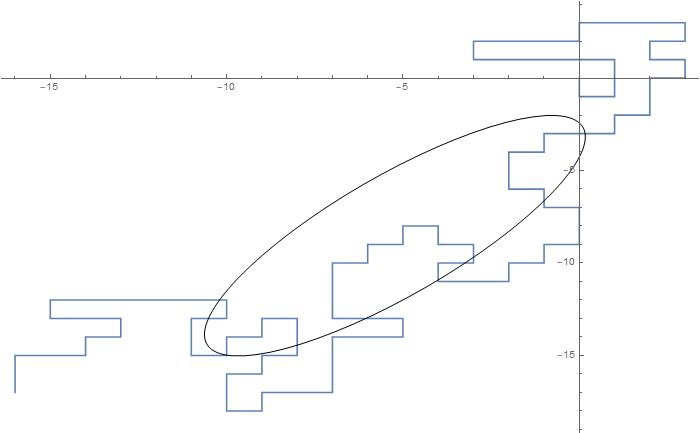
\includegraphics[width=\linewidth]{Sections/Images/GyrationEllipse.png}
\end{minipage}
\hfill
\begin{minipage}[h]{0.5\linewidth}
    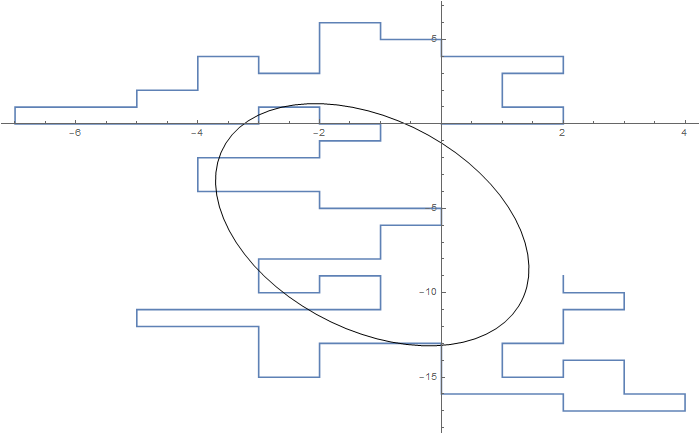
\includegraphics[width=\linewidth]{Sections/Images/GyrationEllipse2.png}
\end{minipage}
\vfill
\begin{minipage}[h]{0.5\linewidth}
     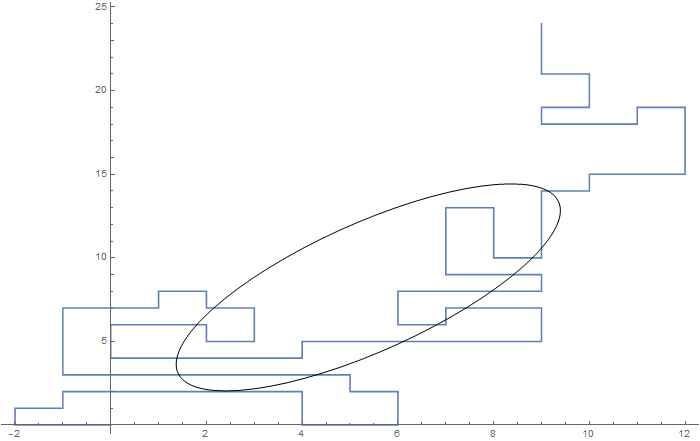
\includegraphics[width=\linewidth]{Sections/Images/GyrationEllipse3.png}
\end{minipage}
\hfill
\begin{minipage}[h]{0.5\linewidth}
    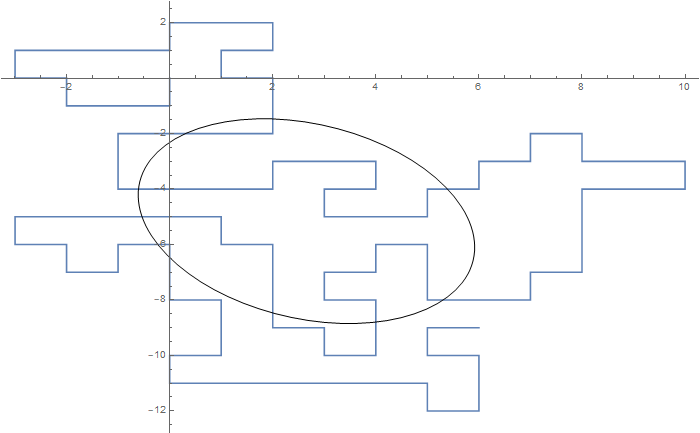
\includegraphics[width=\linewidth]{Sections/Images/GyrationEllipse4.png}
\end{minipage}
    \caption{Примеры работ симуляции по коду из Проект9.pdf\cite{Git}}
    \label{fig:my_label}
\end{figure}


\section{Оценка работы алгоритма для трёхмерной модели Изинга}

\subsection{Расчёт магнитных свойств}

Для первого набора симуляций трёхмерной модели Изинга была расмотрена область J = 0.5 - 0.63 и длины 100-300.

\begin{figure}[!h]
    \centering
    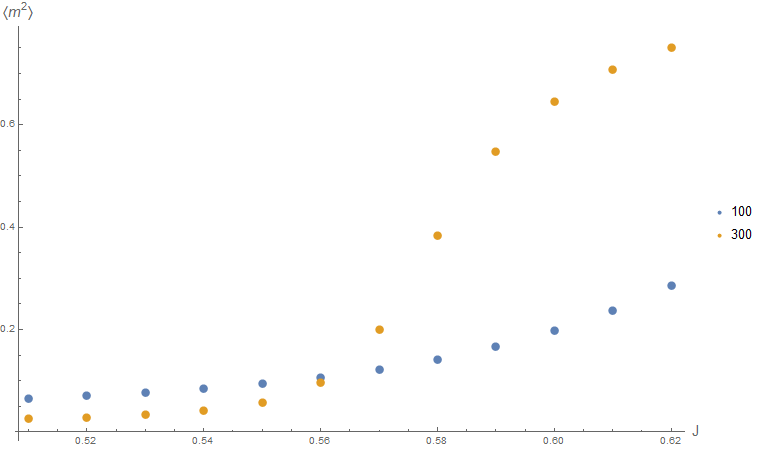
\includegraphics[width=100mm]{Sections/Images/m2_3D_50to60.png}
    \caption{График зависимости квадрата намагниченности от J}
    \label{fig:m2_3D}
\end{figure}

\begin{figure}[!h]
    \centering
    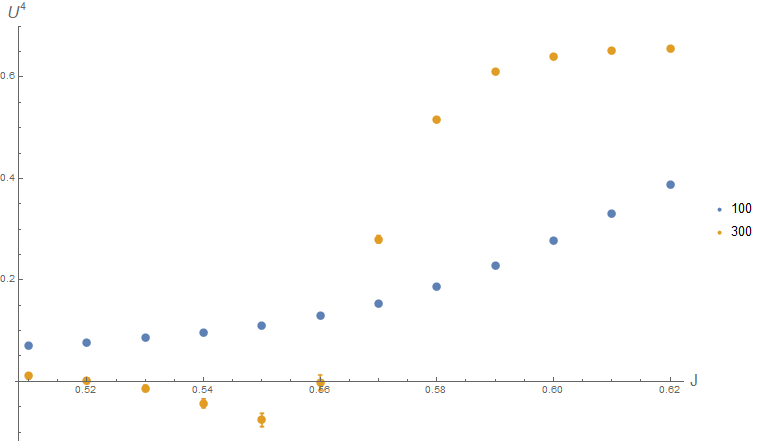
\includegraphics[width=100mm]{Sections/Images/U4_3D_50to60.png}
    \caption{График зависимости значения кумулянта Биндера от J}
    \label{fig:U4_3D}
\end{figure}

Полученные графики подтверждают первичные расчёты Камиллы, в том числе и неясную область отрицательных значений кумулянта Биндера.

\fi

\chapter{3 курс}
\section{Геометрические свойства модели Изинга с точки зрения числа соседей в узлах}

\subsection{Сравнение модели Изинга и полимерной цепочки в решетках с 2-6 возможными соседями у мономеров}

\begin{figure}
    \centering
    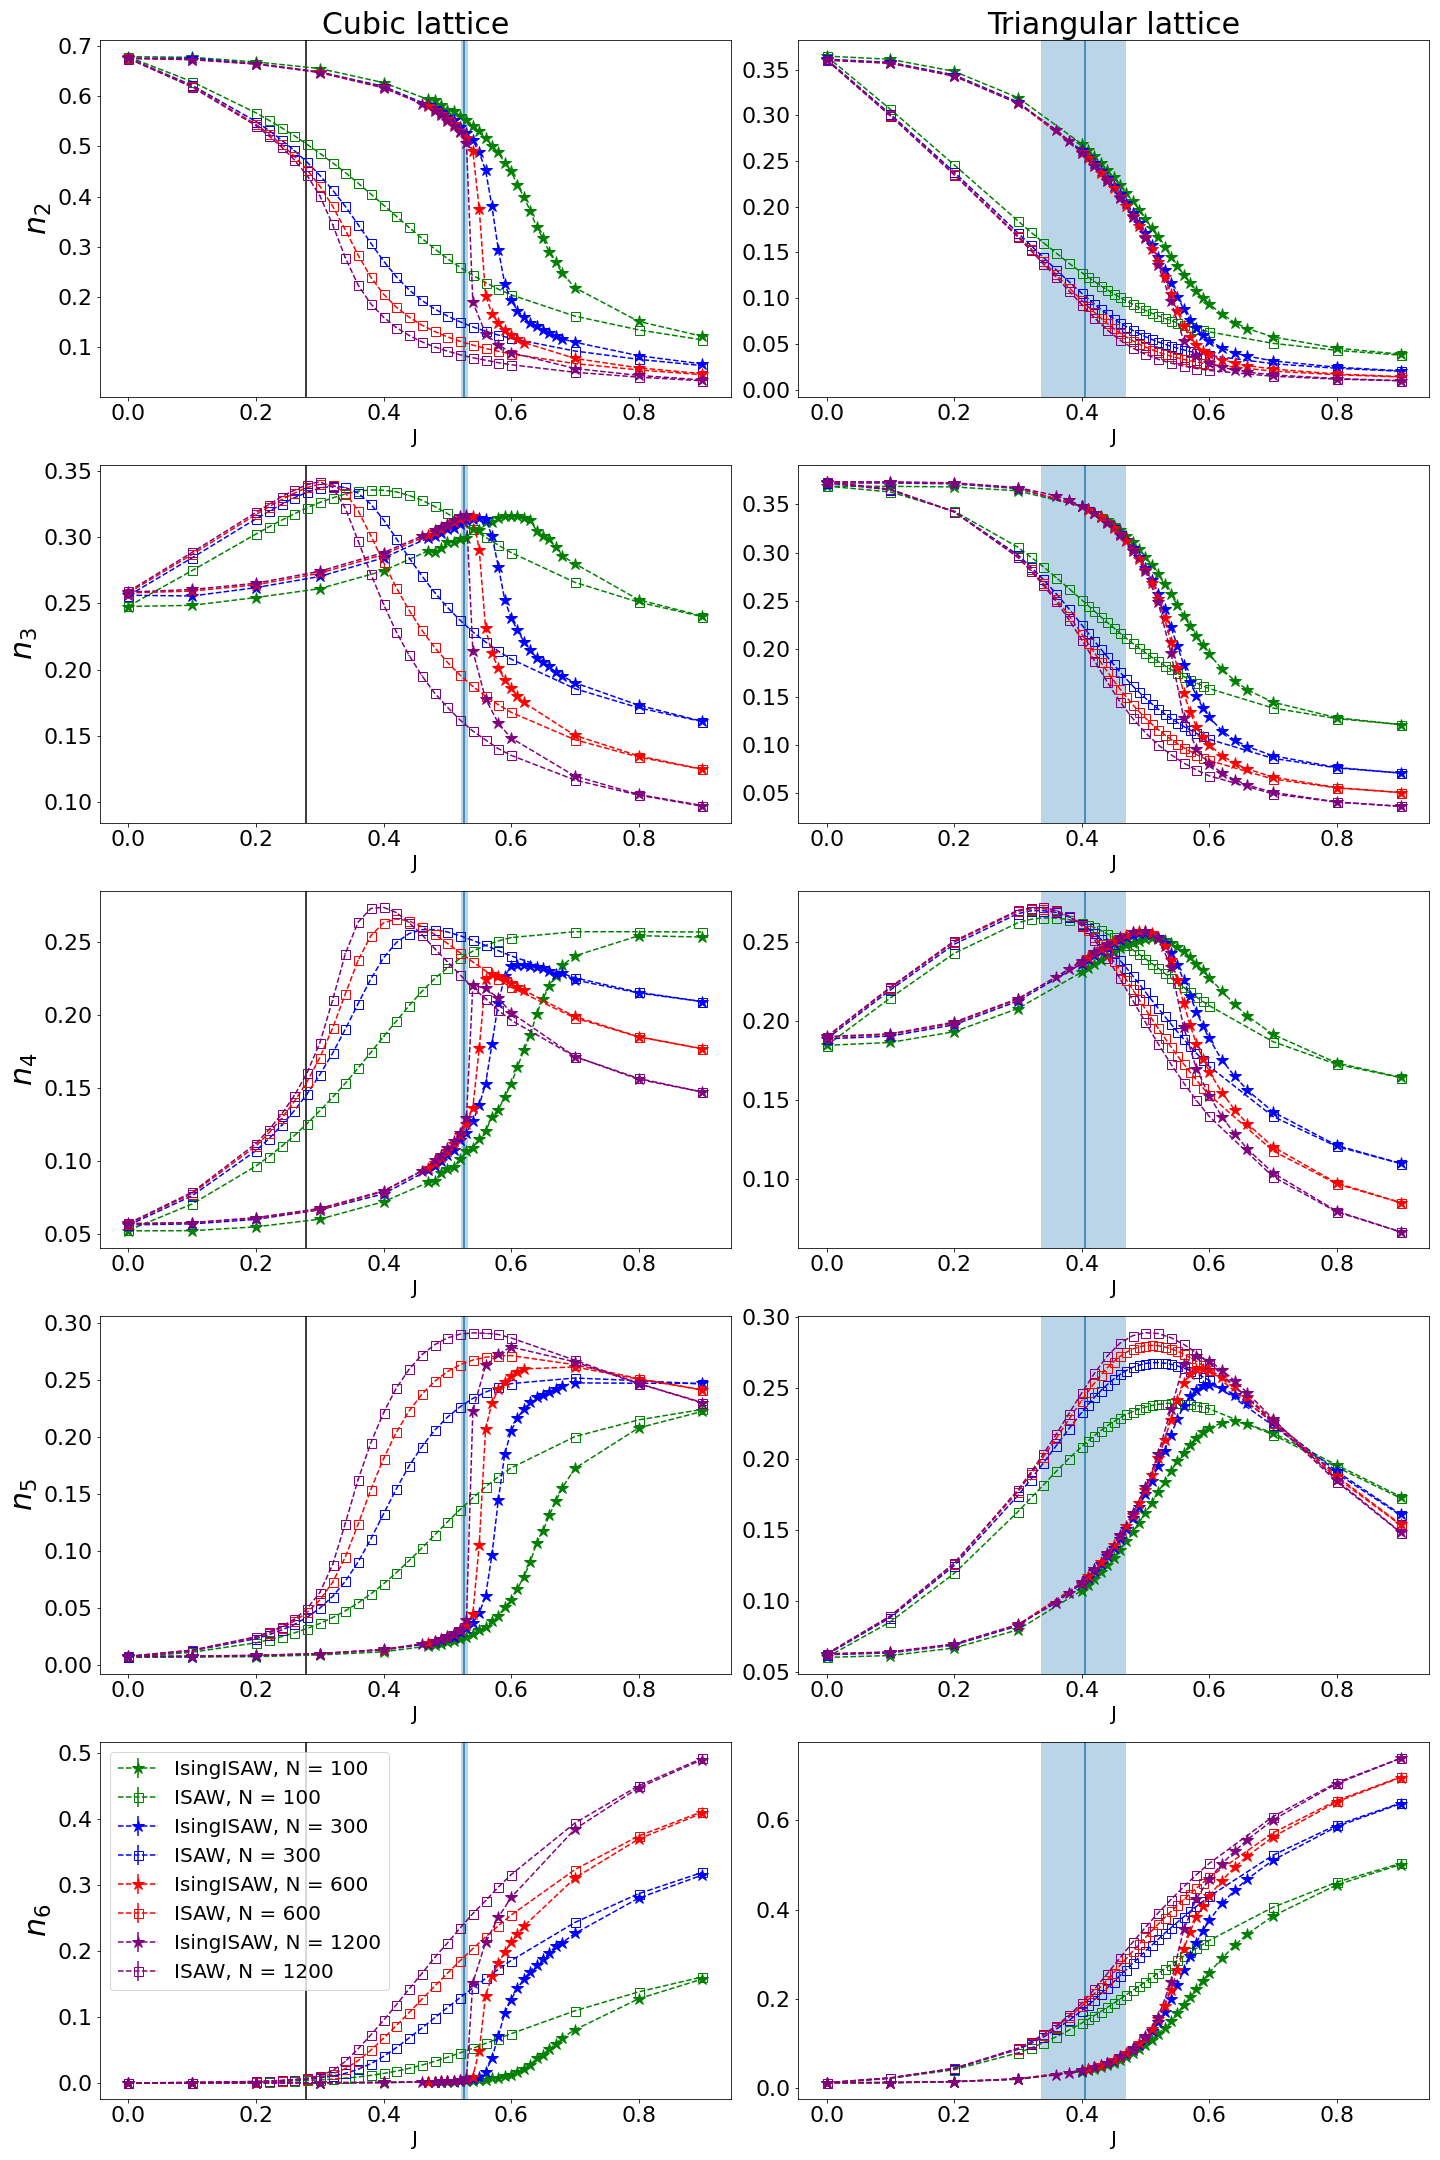
\includegraphics[width=0.95\textwidth, height=21.5cm]{Sections/Images/Ising_vs_ISAW.png}
    \caption{Fractions of monomers of Ising-ISAW model (stars) and ISAW model (open squares) on a cubic lattice (left column) and 2D-triangle lattice (right column) with 2-6 nearest neighbors as function of $J$ with length of conformations $N = $ 100 (green), 300 (blue) and 600 (red). Vertical lines define points of $\theta$-transition (For cubic lattice: black line for ISAW model \cite{Tesi1996} and blue line for Ising-ISAW model \cite{Foster2021}; for triangle lattice: blue line for ISAW model \cite{Privman1986})}
    \label{fig:Ising_vs_ISAW}
\end{figure}

\newpage

\subsection{Сравнение геометрических свойств модели Изинга на треугольной решётке с квадратной}

\begin{figure}
    \centering
    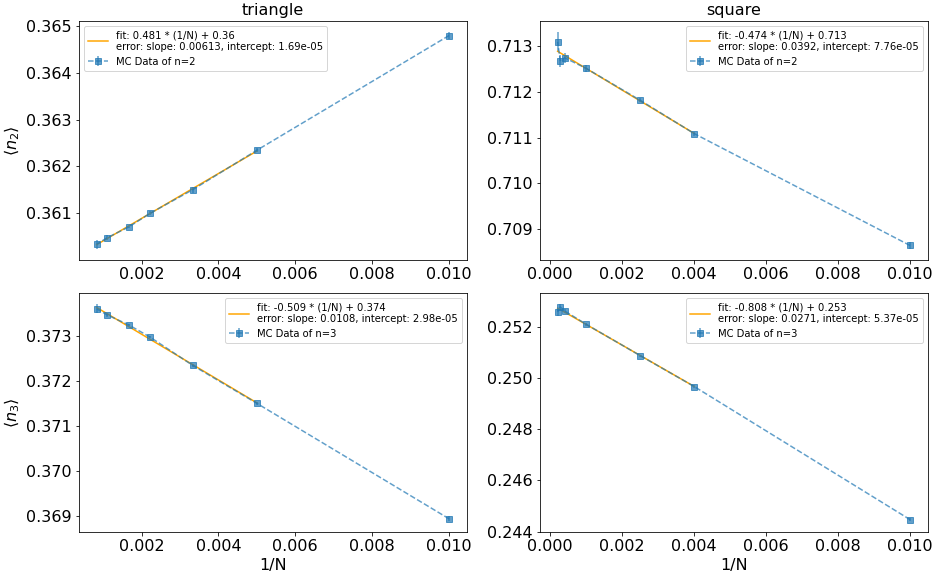
\includegraphics[width=0.95\textwidth]{Sections/Images/triagle_vs_square_bulk.png}
    \caption{Графики зависимости средней доли узлов с 2-3-мя соседями (сверху вниз) от обратной длины 1/N в модели Изинга на треугольной (слева) при N от 200 до 1200 и квадратной (справа) решётках при N от 250 до 4900 при J=0. Синяя линия описывает результаты симуляций Монте-Карло, оранжевая - линейное приближение результатов, ошибки рассчитаны с учётом погрешностей полученных данных}
    \label{fig:tr_vs_sq_bulk}
\end{figure}

На графике \ref{fig:tr_vs_sq_bulk} наглядно показано сравнение приближений долей "одномерных" участков (то есть, долей мономеров с двумя соседями) и узлов с тремя соседями в цепочках на треугольной и квадратной решётках. Для расчётов долей на треугольной решётке были использованы длины 200-1200, для квадратной - 250-4900. Приближение долей треугольной решётки имеет отчётливый линейный характер, включая даже в приближении на всех точках (см. раздел "Подсчёт соседей у треугольной решётки" в Bulk2-6.ipynb\cite{Git}). Линейность долей квадратной решётки также подтверждается (с учётом погрешности расчётов с наибольшей длиной).

Так же хочется заметить некоторое сходство значений свободного члена для долей с двумя соседями и свободного члена в приближениях графика зависимости вероятности гомополимерной цепочки иметь атмосферу 3 в статье Преллберга\cite{Prellberg}, то есть вероятность, что второй конец цепочки длины N имеет 3 возможных направления для удлинения и следовательно, 3 узла, которые могут стать N+1-ым в цепочке.

\begin{table}[]
    \centering
    \begin{tabular}{|c|c|c|c|}
    \hline
    k & $p^{(k)}$ & i & $intercept(\la n_{i} \ra)$ \\ \hline
    3 & 0.711 14(3) & 2 & $0.71299 \pm 2*10^{-5}$ \\ \hline
    2 & 0.225 00(2) & 3 & $0.25291 \pm 10^{-5}$ \\ \hline
    1 & 0.054 76(1) & 4 & $0.03410 \pm 10^{-5}$\\ \hline
    0 & 0.009 096(4) & - & - \\ \hline
    \end{tabular}
    \caption{Таблица сравнения свободных членов линейных приближений вероятностей у конформации иметь n-ю атмосферу (слева) и долей мономеров с i соседями (справа) в зависимости от обратной длины конформации 1/N}
    \label{tab:Prellb_Compare}
\end{table}

На таблице \ref{tab:Prellb_Compare} слева изображены значения свободных членов графика зависимости вероятности гомополимерной цепочки иметь атмосферу k в статье Преллберга\cite{Prellberg}, то есть вероятность, что второй конец цепочки бесконечно большой длины N имеет k возможных направления для удлинения и следовательно, k возможных узлов, которые могут стать новым узлом в цепочке. Справа изображены значения свободных членов приближений графиков долей узлов с i соседями. Хотя все значения отличаются больше чем на погрешность расчётов, однако нельзя не заметить довольно близкое сходство $p^{(3)}$ и свободного члена $\la n_{2} \ra$, хотя сами приближения имеют противоположные по знаку наклоны. 
Возможно, обе величины по-разному описывают одно и то же поведение цепочек с точки зрения их плотности: например, если конец цепочки длины N (назовём его "N-ым узлом") имеет атмосферу три, то при добавлении нового N+1-го узла N-й будет иметь два соседа: N-1-й и N+1-й узлы. Так же при атмосфере 2 (то есть, уже имея два соседа и две возможности для удлинения) N-ый узел при удлинении будет иметь 3 соседа. И наконец, при атмосфере 1 удлинение цепочки приведёт к тому, что старый конец цепочки будет иметь 4 соседа. Очевидно, что случай удлинения при атмосфере 0 рассмореть невозможно, и провести аналогию с соседями нельзя.

Однако сходства между одномерием треугольной и квадратной решётки с точки зрения самих приближений почти не наблюдается - они имеют как разные значения свободных членов, так и значения и даже (в случае 2-х соседей) знаки коэффициента наклона, разница который значительно превышает погрешность фита.



\subsection{Сравнение геометрических свойств модели Изинга на треугольной решётке с кубической}

\begin{figure}
    \centering
    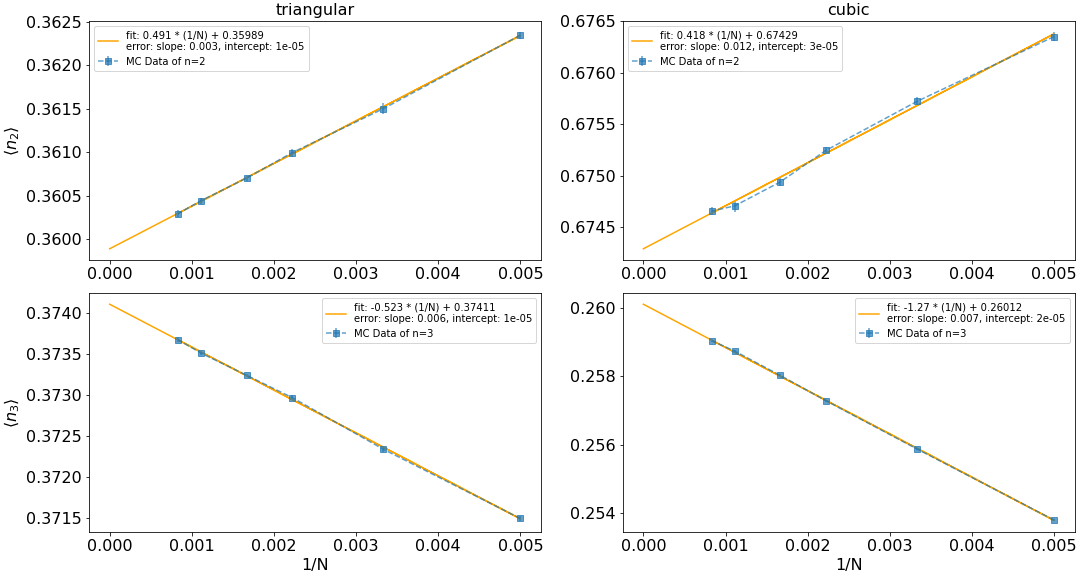
\includegraphics[width=0.95\textwidth]{Sections/Images/triangle_vs_cubic_bulk.png}
    \caption{Зависимость средней доли узлов с 2-3-мя соседями (сверху вниз) от обратной длины 1/N в модели Изинга на треугольной (слева) и кубической (справа) решётках при J=0. Синяя линия описывает результаты симуляций Монте-Карло, оранжевая - линейное приближение результатов, ошибки рассчитаны с учётом погрешностей полученных данных}
    \label{fig:tr_vs_cb_bulk}
\end{figure}

Здесь мы сравниваем линейное приближение треугольной решётки с кубической, имеющейтакое же количество возможных соседей. Получается примерно та же ситуация как и в случае сравнения с квадратной - кубическая решётка на графике \ref{fig:tr_vs_cb_bulk} показывает почти чёткий линейный характер приближения в пределах погрешности наибольших длин (для n=3 линейно видна значительно лучше), но значения не имеют никакого сходства. Единственное отличие от сравнения с квадратной решёткой - графики соответствующих долей имеют одинаковое поведение с точки зрения знака наклона, что действительно и для долей узлов с больший числом соседей. Можно утверждать, что треугольная решётка с точки зрения поведения доли одномерных участок больше похожа на кубическую решётку, нежели квадратную, однако универсальность поведения доли "одномерных" участков среди решёток при бесконечно больших длинах конформации не обнаружена.
\section{Геометрические свойства простого случайного блуждания}

В качестве завершения исследования поведения долей узлов с фиксированным числом соседей рассмотрим модель простого случайного блуждания (далее Random\_Walk или RW) на квадратной решётке. 
В модели RW отсутствует ограничение самопересечений, и, следовательно, есть возможность попадания в ранее занятые узлы решётки.

Определим два геометрических свойства конформаций модели RW: из семейства SAW-моделей взято \textit{количество шагов блуждания} $N$. 
Оно является параметром модели, и при генерации блужданий все конформации имеют фиксированное количество шагов.
Добавляется новая наблюдаемая величина -- \textit{доля уникальных узлов блуждания} $\nun$ -- отношение количества занятых блужданием узлов $\Nun$ к количеству шагов $N$.

\begin{equation}
\nun = \frac{\Nun}{N}
\label{eq:nun}
\end{equation}

Как и в предыдущих разделах, исследуемыми свойствами будут величины $n_i, i \in \{1..4\}$ -- \textit{доли узлов с фиксированным числом соседей}. 
Так же будет рассмотрена атмосфера блужданий модели RW -- \textit{число незанятых узлов решётки вокруг конца блуждания}. 
В частности, исследуется поведение вероятности $\pkn$ -- доли конформаций из N шагов с атмосферой $k \in \{0..3\}$ среди сгенерированных -- с увеличением количества шагов $N$.
Доли $n_i$ и, конечно, атмосфера $k$, считаются сразу среди уникальных узлов сгенерированной конформации, для чистоты результатов и возможности сравнения с данными исследования случайного блуждания без самопересечений.
Все величины будут рассмотрены в виде двух функций:

\begin{itemize}
\item Доли узлов как функция количества шагов простого случайного блужания $N$: 
\begin{equation}
 \la n_i \ra = f_i(N),\ \ \ \ i \in \{1,2,3,4, \textup{unique}\}
\label{eq:f_i}
\end{equation}
\item Доли узлов как функция количества уникальных узлов блуждания $\Nun = N \nun$:
\begin{equation}
 \la n_i \ra = g_i(\Nun),\ \ \ \ i \in \{1,2,3,4\} 
\label{eq:g_i}
\end{equation}
\end{itemize}

Основными целями раздела будут:

\begin{enumerate}
\item Определение характера шкалирования наблюдаемых величин при бесконечно большом блуждании ($N \to \infty,\ \Nun \to \infty$)
\item Оценка коэффициетов фитирующих функций $f_i, g_i$, в особенности - асимтотического предела наблюдаемых
\item Для проверки результатов: численное сравнение фитирующих функций при прямой зависимости от кол-ва шагов $f_i(N)$ и сложной зависимости от $\Nun$, которое, в свою очередь, зависит от $N$ $g_i(f_{\textup{unique}}(N))$
\end{enumerate}



\begin{figure}[h]
    
\begin{subfigure}{0.5\textwidth}
    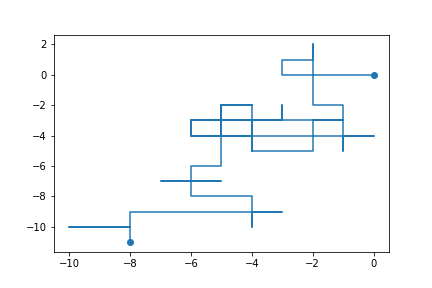
\includegraphics[width=\textwidth]{Rand_Path.png}
    \caption{}
    \label{fig:path_1}
\end{subfigure}
\hfill
\begin{subfigure}{0.5\textwidth}
    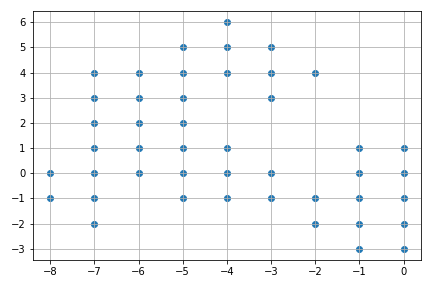
\includegraphics[width=\textwidth]{Rand_Path_Unique.png}
    \caption{}
    \label{fig:path_2}
\end{subfigure}
\vfill
\centering
\begin{subfigure}{0.5\textwidth}
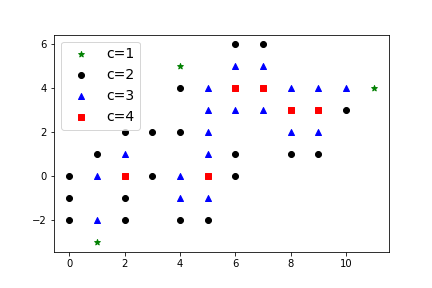
\includegraphics[width=\textwidth]{Rand_Path_Neigh.png}
\caption{}
\label{fig:path_3}
\end{subfigure}
\caption{а) Сгенерированное блуждание модели RW $\{\omega_i\}$ \eqref{eq:DS_alg} из $N$ шагов. Концы блуждания отмечены жирными точками, ходы блуждания -- линией. Началом блуждания является зелёная точка $(0,0)$, концом блуждания -- черная, в которой так же рассчитывается атмосфера блужания $k$. б) Набор уникальных точек $\{\omega^u_i\}$ \eqref{eq:w_u}, принадлежащих блужданию модели RW, количество которых -- $\Nun$. в) Подсчёт соседей у каждого узла блуждания. Доля узлов с k соседей считается по формуле \eqref{eq:n_i}.}
\end{figure}

\subsection{Алгоритм генерации блужданий}

Блуждания $\{ \omega_ i \}$ генерируются в виде последовательности индексов направлений $ \{d_{i}\} $ в любой решётке, что ускоряет процесс моделирования. 
Первая точка блуждания на решётке $\omega_{0}$ лежит в начале координат $(0,0)$, далее блуждание определяется как последовательность узлов по формуле \eqref{eq:DS_alg}:
\begin{equation}
\{ \omega_i \} = 
\begin{cases}
\omega_{0} = (0,0) \\
\omega_{i} = \omega_{i-1} +\textup{steps}\left[d_{i}\right] 
\end{cases}
\begin{array}{l}
\textup{steps} = \left[(0,1), (0,-1), (1,0), (-1,0)\right], \\
d_i = \textup{Random}(\{0,1,2,3\}), i = 1..N,
\end{array}
\label{eq:DS_alg}
\end{equation}
где steps - массив фиксированных смещений из точки, определяемые законами решётки. 
Точность подсчёта наблюдаемых определяется лишь количеством повторов эксперимента.

С другой стороны, отсутствие требования непересекаемости блуждания вызывает ряд осложнений для сравнения результатов с классом блужданий без самопересечений. 
Например, возможны случаи, когда два идущих подряд направления противоположны друг другу - то есть, на i-м шаге блуждание смещается из точки $\omega_{i-1}$, а i+1-м - возвращается в него, то есть $\omega_{i-1} = \omega_{i+1}$.
В таком случае на графике блуждания возможны ''шипы'', концы которых будут узлами с всего одним соседом - основанием ''шипа''. 



Алгоритм обработки каждого модерируемого блуждания описан на картинках \ref{fig:path_1}, \ref{fig:path_2} и \ref{fig:path_3}:
\begin{itemize}
    \item Из сгенерированного блуждания (рисунок \ref{fig:path_1}) отбираются все уникальные точки узлов \eqref{eq:w_u} - образуется набор точек решётки $\{\omega^u_i\}, i = \{0, \Nun-1\}$ (рисунок \ref{fig:path_2}). Так же считается доля уникальных узлов блуждания \eqref{eq:nun}.
	\begin{equation}
	\begin{array}{l}
	\{ \omega^u_i \} = \textup{Unique}( \{ \omega_i \} ) \\
	N_{\textup{unique}} = |\{ \omega^u_i \}|
	\end{array}
	\label{eq:w_u}
	\end{equation}
    \item Для каждого уникального узла рассчитывается кол-во его соседей $c_i \in \{1,2,3,4\}$  (рисунок \ref{fig:path_3}).
    \item Доля узлов с k соседями считается как отношение количества уникальных узлов с k соседями к общему количеству уникальных узлов.
	\begin{equation}
	n_k = \frac{\sum_{i=0}^{\Nun-1}[c_i = k]}{\Nun}
	\label{eq:n_i}
	\end{equation}
\end{itemize}

\subsection{Результаты симуляций}

Была проведена генерация модели RW с количеством шагов $N = 10^{2}-10^{4}$. 
Доли уникальных узлов $\nun$ так же брались во внимание при симуляциях. 
Результаты симуляций, а так же количество итераций для каждой длины, описаны в таблице \ref{tab:Ran_Walk_neigh} и изображены на графиках \ref{fig:DS_n_i}, \ref{fig:DS_n_iu} и \ref{fig:DS_n_u}.\footnotemark{}.\footnotetext{Процесс симуляций был запрограмирован на языке Python и проводился с использованием суперкомпьютера НИУ ВШЭ. Оптимизация требовала дополнительного изменения окружения - см. технический раздел \ref{subsection:njit_problem}}

В следующих подразделах будет проведён анализ полученных результатов - сначала будет проведено обсуждение погрешностей данных, затем - оценка и сравнение шкалирующих функций \eqref{eq:f_i}, \eqref{eq:g_i} для наблюдаемых величин.

\begin{table}[h]
    \centering

\begin{tabular}{|c|c|c|c|c|c|c|}
\hline
N & steps & $ \nun $ & $n_{1}$ & $n_{2}$ & $n_{3}$ & $n_{4}$ \\ \hline
100 & 96430000 & 0.490868(8) & 0.067676(3) & 0.33516(1) & 0.357310(7) & 0.239851(9) \\ \hline
150 & 69360000 & 0.462622(9) & 0.057825(3) & 0.30787(1) & 0.356280(7) & 0.27802(1) \\ \hline
200 & 36140000 & 0.44436(1) & 0.052236(4) & 0.29043(1) & 0.353706(9) & 0.30362(2) \\ \hline
350 & 17070000 & 0.41251(2) & 0.043761(4) & 0.26070(1) & 0.34590(1) & 0.34963(2) \\ \hline
500 & 7720000 & 0.39439(2) & 0.039590(5) & 0.24424(2) & 0.33965(2) & 0.37652(3) \\ \hline
750 & 4810000 & 0.37559(2) & 0.035672(5) & 0.22759(2) & 0.33188(2) & 0.40487(4) \\ \hline 
1000 & 2480000 & 0.36325(3) & 0.033333(6) & 0.21696(3) & 0.32610(2) & 0.42361(5) \\ \hline
3000 & 420000 & 0.32265(6) & 0.02650(1) & 0.18336(5) & 0.30351(5) & 0.4865(1) \\ \hline
5000 & 140000 & 0.30679(9) & 0.02434(1) & 0.17086(8) & 0.29322(8) & 0.5116(2) \\ \hline
6500 & 100000 & 0.2992(1) & 0.02330(2) & 0.16518(9) & 0.28816(9) & 0.5234(2) \\ \hline
7000 & 305000 & 0.29610(6) & 0.02302(1) & 0.16340(5) & 0.28657(5) & 0.5270(1) \\ \hline
8000 & 240000 & 0.29338(6) & 0.02253(1) & 0.16070(5) & 0.28409(6) & 0.5327(1) \\ \hline
9000 & 195000 & 0.29022(7) & 0.02215(1) & 0.15830(6) & 0.28185(6) & 0.5377(1) \\ \hline
10000 & 160000 & 0.28751(8) & 0.02179(1) & 0.15628(6) & 0.27991(7) & 0.5420(1) \\ \hline
\end{tabular}

    \caption{Средние доли узлов c 1-4-мя (столбцы $n_1$-$n_4$) соседями, а так же доля уникальных узлов (столбец $\nun$) в конформациях модели Random-Walk длин $10^{2}$-$10^{4}$ (столбец $N$). Также изображены на графиках \ref{fig:DS_n_i}, \ref{fig:DS_n_iu} и \ref{fig:DS_n_u}. В столбце steps выписано количество итераций алгоритма Монте-Карло.}
    \label{tab:Ran_Walk_neigh}
\end{table}

\begin{figure}[h]

\begin{subfigure}{0.5\textwidth}
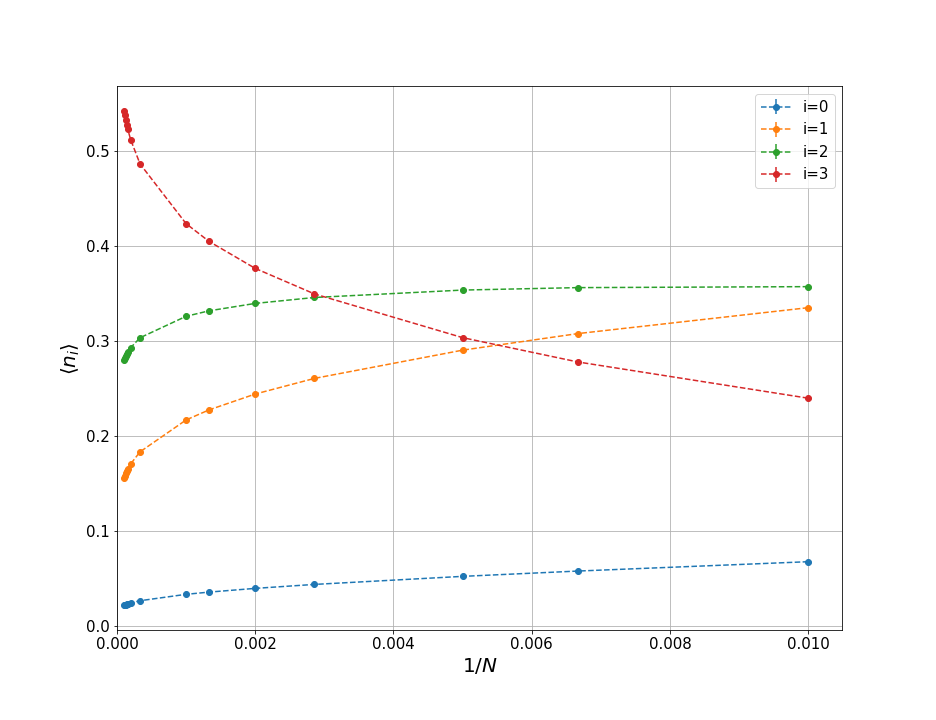
\includegraphics[width=\textwidth]{Rand_Path_n_i.png}
\caption{}
\label{fig:DS_n_i}
\end{subfigure}
\hfill
\begin{subfigure}{0.5\textwidth}
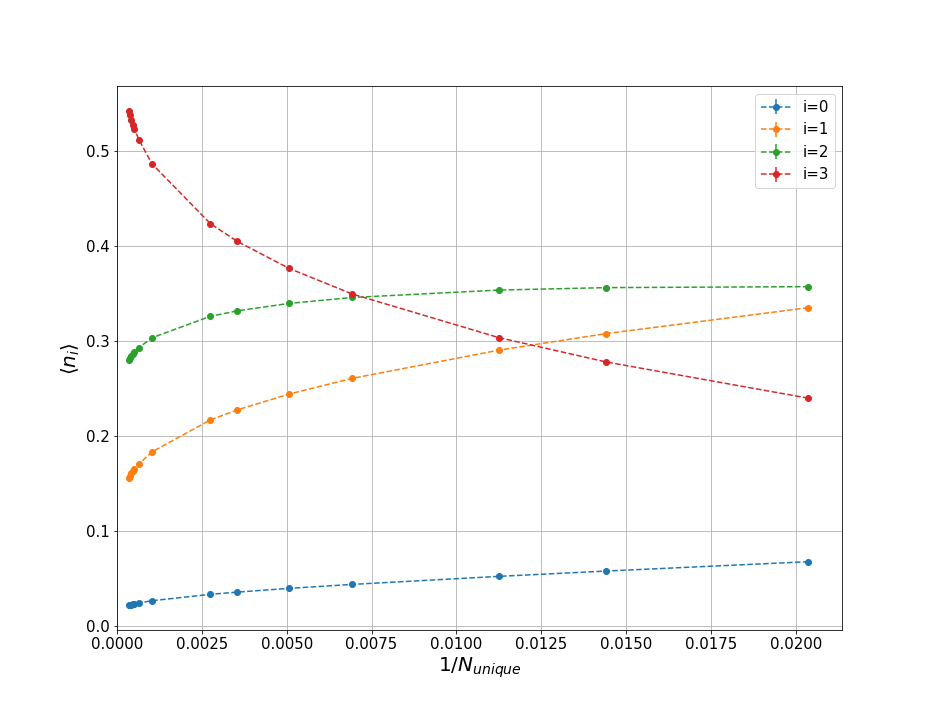
\includegraphics[width=\textwidth]{Rand_Path_n_i_unique.png}
\caption{}
\label{fig:DS_n_iu}
\end{subfigure}
\vfill
\centering
\begin{subfigure}{0.5\textwidth}
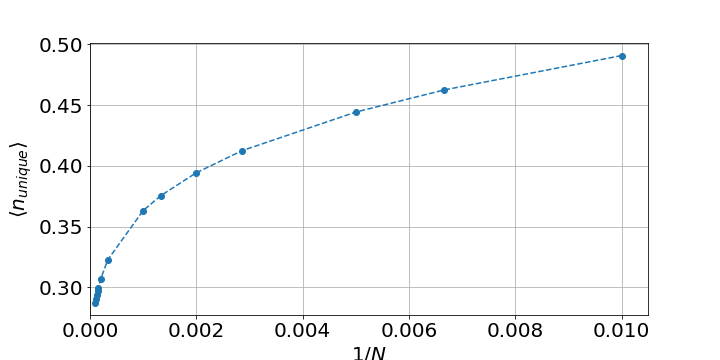
\includegraphics[width=\textwidth]{Rand_Path_n_unique.png}
\caption{}
\label{fig:DS_n_u}
\end{subfigure}
\caption{Доли узлов с фиксированным числом соседей (столбцы $n_1$-$n_4$ из таблицы \ref{tab:Ran_Walk_neigh}): а) от обратного количества шагов блуждания $1/N$; b) обратного количества уникальных узлов $1/\Nun$; c) Доли уникальных узлов (столбец $\nun$ из таблицы \ref{tab:Ran_Walk_neigh}) от обратного количества шагов блуждания $1/N$. }
\end{figure} 

\newpage

\subsection{Погрешности результатов}

Полученные в данной подсекции результаты имели ранее необоснованно большие погрешности, что потребовало более тщательного исследования. 
Необходимо проверить распределение результатов со временем, а так же сходимость средних наблюдаёмых величин и их ошибок.
 В качестве примера рассмотрим первую исследуемую длину $N=100$, т.к. именно её симуляции протекают быстрее всех.  

Распределение наблюдаемых долей узлов с фиксированным числом соседей 1-4, а так же доли уникальных узлов рассмотрены на гистограммах на левом графике рисунка \ref{fig:DS_100_dists_history}  в двух моментах времени: после $10^6$ шагов и после $2.5 \cdot 10^6$  шагов. 
На рисунке видно, что данные всех величин имеют нормальное или близко к нормальному распределению, а несимметричные склоны  некоторых величин ($n_1$ и $n_2$) объясняются близостью соответствующего края к нулю.

Сходимость наблюдаемых величин можно увидеть на правом графике \ref{fig:DS_100_dists_history}, где замеры средних проводились через каждые 4000 шагов. На графике средних заметна сходимость средней величины и уменьшение колебаний. 
С другой стороны, график среднего квадратического отклонения не стремится к нулю как ожидалось, а так же сходится с уменьшением колебаний к ненулевому значению. 
Это показывает противоречивость результатов (по крайней мере замеров ошибки - среднее явно сходится), причину чему следует искать в коде. 

Для удостоверения, что причина не лежит в jit-компиляции, был проведён запуск нескомпилированного с помощью numba кода. Результаты оказались идендичны с jit-компиляцией, и следовательно проблема в другом месте.

\begin{figure}
	\caption{Слева: Распределение долей узлов с 1-4 соседями и уникальных узлов блуждания длины 100 в два момента времени. Справа: История результатов (Столбец mean - средняя величина, столбец std - значение ошибки на i-м замере) долей узлов с 1-4 соседями и уникальных узлов блуждания длины 100 с интервалом замеров в 4000 шагов.}
     \label{fig:DS_100_dists_history}
\begin{minipage}{0.32\textwidth}
     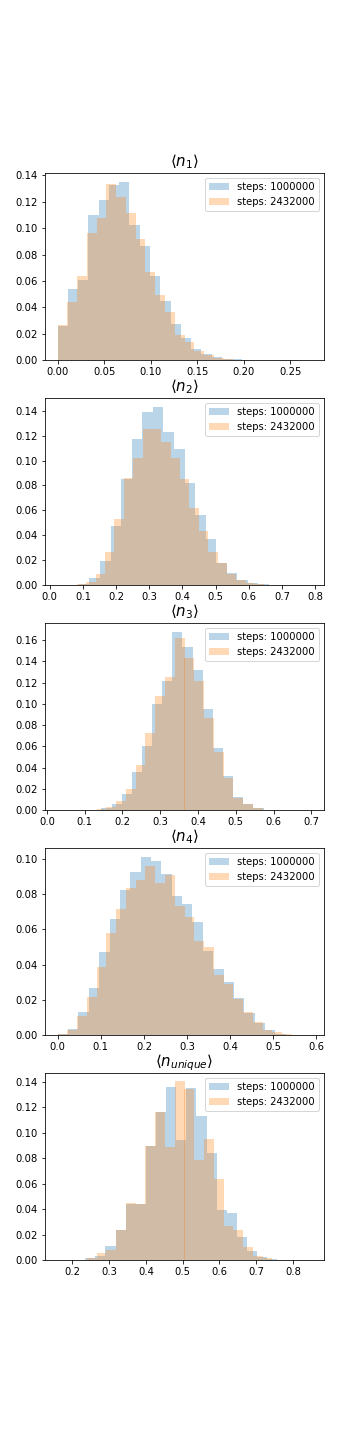
\includegraphics[width=\textwidth]{DS_100_dists.png}
\end{minipage}
\begin{minipage}{0.67\textwidth}
     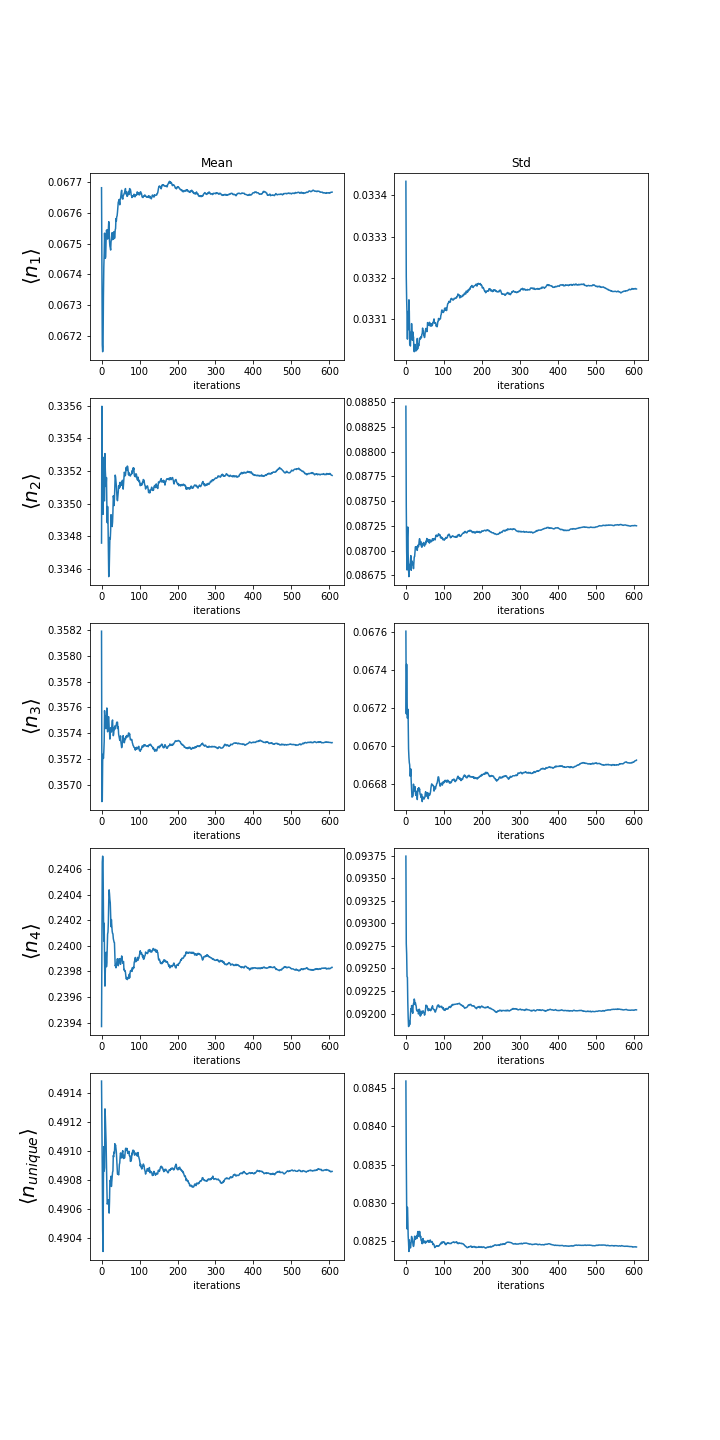
\includegraphics[width=\textwidth]{DS_100_history.png}
\end{minipage}
	
\end{figure}


Причиной столь больших погрешностей результатов была неверная интерпретация понятия "ошибка среднего", толковавшаяся ранее, как выборочное среднее квадратическое отклонение $\sigma(x)$ результатов симуляций $x$ - на деле ошибкой среднего является формула вида:

\[\Delta\la x \ra = \sigma(x)/\sqrt{N},\]

где  $N$ - объём выборки или количество экспериментов.


\subsection{Шкалирование результатов}

Применим к результатам из таблицы \ref{tab:Ran_Walk_neigh} те же методы анализа, что и ранее для доли узлов с фиксированным числом соседей в СБС -- определим характер шкалирования долей при стремлении длины конформации модели RW к бесконечности.
Рассмотрим данные в трёх предполагаемых масштабах: в линейной, лог-линейной и лог-логарифмической масштабностях от обратной длины $1/N$ и кол-ва уникальных узлов $1/\Nun$.
Пример исследуемых данных показан на графике \ref{fig:n1_scale}. 
На нём видно, что в случае лог-лог-шкалирования (или степенного) график обретает наилучшую среди трёх масштабностей линейность.
Оно же оказолось наиболее подходящим в графиках всех долей узлов $n_{1-4}$ в обоих функциях $f_i(N), g_i(\Nun)$, а так же для зависимости $\nun$ от кол-ва шагов $N$.

\begin{figure}
\centering
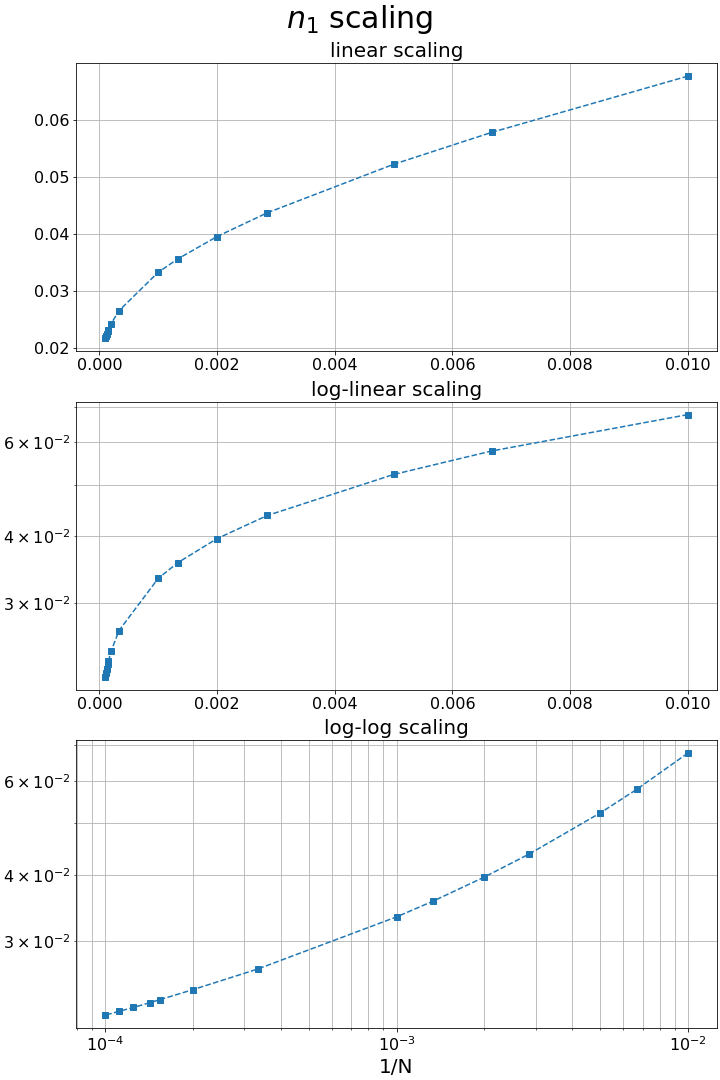
\includegraphics[width=0.7\textwidth]{n1_res.png}
\caption{Зависимость $n_1$ от $1/N$  в линейной, лог-линейной и лог-логарифмической масштабностях (сверху-вниз), по данным из таблицы \ref{tab:Ran_Walk_neigh}.} 
\label{fig:n1_scale}
\end{figure}

Тогда, шкалирующая функция $f_i(N)$ рассматривается в виде:

\begin{equation}
f_i(N) = k_i (1/N)^{a_i} + b_i,\ \ \ i \in \{1,2,3,4, \textup{unique}\}
\label{eq:n_i_log_log}
\end{equation}

Полученные коэффициенты с погрешностями выписаны на таблице \ref{tab:n_i_log_log}.

\begin{table}[h]
\centering
\begin{tabular}{|c|c|c|c|c|}
\hline
 & k & a & b & N \\ \hline
$n_1$ & 0.3425(8) & 0.417(2) & 0.014(1) & 3000-10000 \\ \hline
$n_2$ & 0.573(4) & 0.171(1) & 0.037(2) & 3000-10000 \\ \hline
$n_3$ & 0.588(3) & 0.219(3) & 0.202(3) & 3000-10000 \\ \hline
$n_4$ & -1.239(9) & 0.189(3) & 0.759(5) & 500-10000 \\ \hline
$n_{unique}$ & 0.831(1) & 0.2049(2) & 0.1616(4) & 500-10000 \\ \hline
\end{tabular}
\caption{Коэффициенты степенной шкалирующей функции доли узлов от обратного количества шагов блуждания $1/N$ \eqref{eq:n_i_log_log}.}
\label{tab:n_i_log_log}
\end{table}
Аналогичный анализ проведён для зависимости долей узлов $n_1 - n_4$ от количества уникальных узлов $\Nun$:

\begin{equation}
g_i (\Nun) = q_i  (1/\Nun)^{s_i} + d_i,\ \ \ i \in \{1,2,3,4\}
\label{eq:n_i_u_log_log}
\end{equation}

\begin{table}[h]
\centering
\begin{tabular}{|c|c|c|c|c|}
\hline
 & q & s & d & $\Nun$ \\ \hline
$n_1$ & 0.313(1) & 0.479(2) & 0.015(1) & 967-2875 \\ \hline
$n_2$ & 0.567(3) & 0.214(1) & 0.053(2) & 967-2875 \\ \hline
$n_3$  & 0.542(5) & 0.244(2) & 0.203(2) & 967-2875 \\ \hline
$n_4$ & -1.20(1) & 0.225(4) & 0.741(5) & 197-2875 \\ \hline
\end{tabular} 
\caption{Коэффициенты степенной шкалирующей функции доли узлов от обратного количества уникальных узлов блуждания $1/N_{unique}$ \eqref{eq:n_i_u_log_log}.}
\label{tab:n_i_u_log_log}
\end{table}

\newpage 
\subsubsection{Зависимость доли уникальных узлов от количества шагов}

В данном подразделе проверяется численная эквивалентность фитирующих функций долей узлов $n_1-n_4$: $f_i$ \eqref{eq:n_i_log_log}, имееющей прямую зависимость от числа шагов $N$ и $g_i(\Nun)$ \eqref{eq:n_i_u_log_log}, со сложной зависимостью от $N$.

Рассмотрим аппроксимацию произвольной функции $g_i(\Nun)$ с выражением её аргумента через $N$. Определелим её коэффициенты как $k_i, a_i, b_i$:

\begin{equation}
	\la n_i \ra = g_i(\Nun) = k_i * (1/\Nun)^{a_i} + b_i
	\label{eq:gi_approx1}
\end{equation}

Из результатов прошлого подраздела были получены коэффициенты фитирующей функции $\nun$ (строка $\nun$ таблицы \ref{tab:n_i_log_log}). Определим их как $k_u, a_u, b_u$ соответственно и раскроем их в функции аргумента: 

\begin{equation}
	\Nun = N \nun(N) = N (k_u (1/N)^{a_u} + b_u)
	\label{eq:gi_appprox2}
\end{equation}


Подставим \eqref{eq:gi_appprox2} в \eqref{eq:gi_approx1} и проведём линеаризацию результата в два шага - сначала $1/\Nun$, а затем $(1/\Nun)^{a_i}$:

\begin{large}
\begin{equation*}
\begin{array}{l}
1)\ \ \ \ \ (N (b_u + k_u(1/N)^{a_i})^{-1} = ( N b_u)^{-1} (1 + \frac{k_u}{b_u} (\frac{1}{N})^{a_u})^{-1} = \frac{1}{b_u N} (1 - \frac{k_u}{b_u} (\frac{1}{N})^{a_u} + O(\left(\frac{1}{N})^{2a_u})\right) \\

2)\ \ \ \ \ ( - // - )^{a_i}  = (\frac{1}{b_u N})^{a_i} * (1 - \frac{k_u}{b_u} (\frac{1}{N})^{a_u} + O(\left(\frac{1}{N}\right)^{2a_u}))^{a_i} =  (\frac{1}{b_u N})^{a_i} * (1 - \frac{k_u a_i}{b_u} (\frac{1}{N})^{a_u} + O(\left(\frac{1}{N}\right)^{2a_u}))
\end{array}
\end{equation*}
\end{large}

Итоговое выражение примет следующий вид:

\begin{large}
\begin{equation}
g_i(N) = \frac{k_i}{b_u^{a_i}} (\frac{1}{N})^{a_i} - \frac{k_i a_i k_u}{b_u^{a_i+1}} (\frac{1}{N})^{a_u+a_i} + b_i + O((\frac{1}{N})^{2 a_u +a_i}),\ \ \ \ \ N \to \infty
\end{equation}
\label{eq:g_n_expect}
\end{large}

Таким образом, мы свели функцию $g_i(\Nun)$ \eqref{eq:gi_approx1} к функции вида \eqref{eq:n_i_log_log}, сохранив дополнительные степенные поправки. 
Очевидно, линеризация повлияет на поведение в функции области небольших длин блуждания, поэтому оценивать теорически ожидаемые линейный и степенной коэффициент по полученной функции \eqref{eq:g_n_expect} невозможно.
Это объясняет различие коэффициетов $k_i, a_i$ 

С другой стороны, проведенные преобразования не дали никакой поправки для асимптотического предела $b_i$ - следовательно, вне зависимости от взятого аргумента, $N$ или $\Nun$, функции соответствующих долей узлов с фиксированным числом соседей $f_i$ и $g_i$ должны сходиться на бесконечности в одной точке, а столбцы $b_i$ таблиц \ref{tab:n_i_log_log} \ref{tab:n_i_u_log_log} - равными в пределах погрешностей.
Это так же подтверждается тем, что если $N \to \infty$, то и, очевидно $\Nun \to \infty$, поскольку $b_u > 0$.  

Рассмотрим графики трёх функций на каждую долю $n_1 - n_4$: как функцию $f_i(N)$, как функцию $g_i(N*\nun(N))$, а так же аппроксимацию второй функции \eqref{eq:g_n_expect}.

Графики функций в линейном масштабе изображены на рисунке \ref{fig:ni_fn_vs_gNun}. По ним видно, что функция $f(N)$ и $g(\Nun(N))$ почти не имеют отличий, что говорит о полном взаимозаменяемости аргументов и правильности полученных результатов на небольших длинах. Зелёная линия соответствует аппроксимирующему виду $g(\Nun(N))$ и имеет поправку, уменьшающуюся при стремлении $N$ к бесконечности, но так же визуально сливается с первыми двумя функциями в области больших $N$.

\begin{figure}
\centering
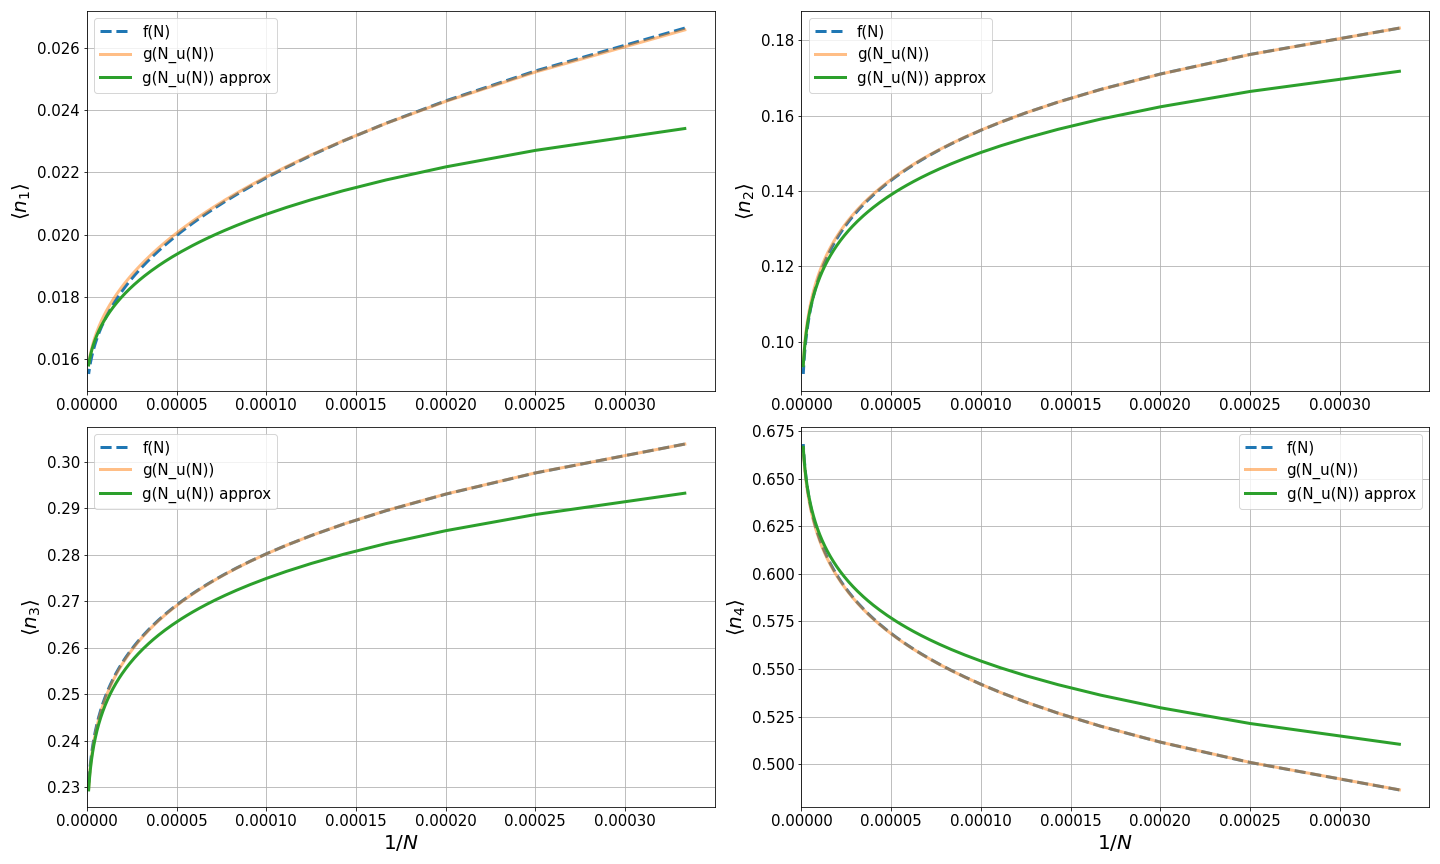
\includegraphics[width=\textwidth]{n_i_fN_vs_gNun.png}
\label{fig:ni_fn_vs_gNun}
\caption{Доли узлов $n_1-n_4$ в линейном масштабе как функции от количества шагов (синий пунктир) \eqref{eq:n_i_log_log}, а так же сложные функции от количества уникальных узлов от количества шагов (оранжевая линия - прямая подстановка функций  \eqref{eq:gi_appprox2} в \eqref{eq:gi_approx1}, зелёная - аппроксимация \eqref{eq:g_n_expect}), по горизонтали - обратное количество шагов блуждания $1/N$. Коэффициеты взяты из таблиц \ref{tab:n_i_log_log} и \ref{tab:n_i_u_log_log}}
\end{figure}

Логарифмический масштаб графиков представлен на рисунке \ref{fig:ni_fn_vs_gNun_log}. 
Здесь ситуация выглядит совершенно иначе: на всех графиках наблюдается расхождение $f_i$ и $g_i$ по мере сближения с нулём.
Причём теперь $g_i$ и её аппроксимация сливаются в одну кривую (что говорит о правильности полученной линеризацией функции \eqref{eq:g_n_expect}). 
Из прошлого раздела мы узнали, что асимпотические пределы $n_1$ и $n_3$ равны в пределах погрешности между выбранными зависимостями.

Однако пределы двух других функций как численно, так и графически расходятся между $f_i$ и $g_i$, что противоречит предположениям о связи зависимостей в пределе бесконечного числа шагов блуждания.
Из возможных причин такого явления не проверен технический аспект фитирования методом наименьших квадратов, а именно зависимость результатов от стартового положения.


\begin{figure}
\centering
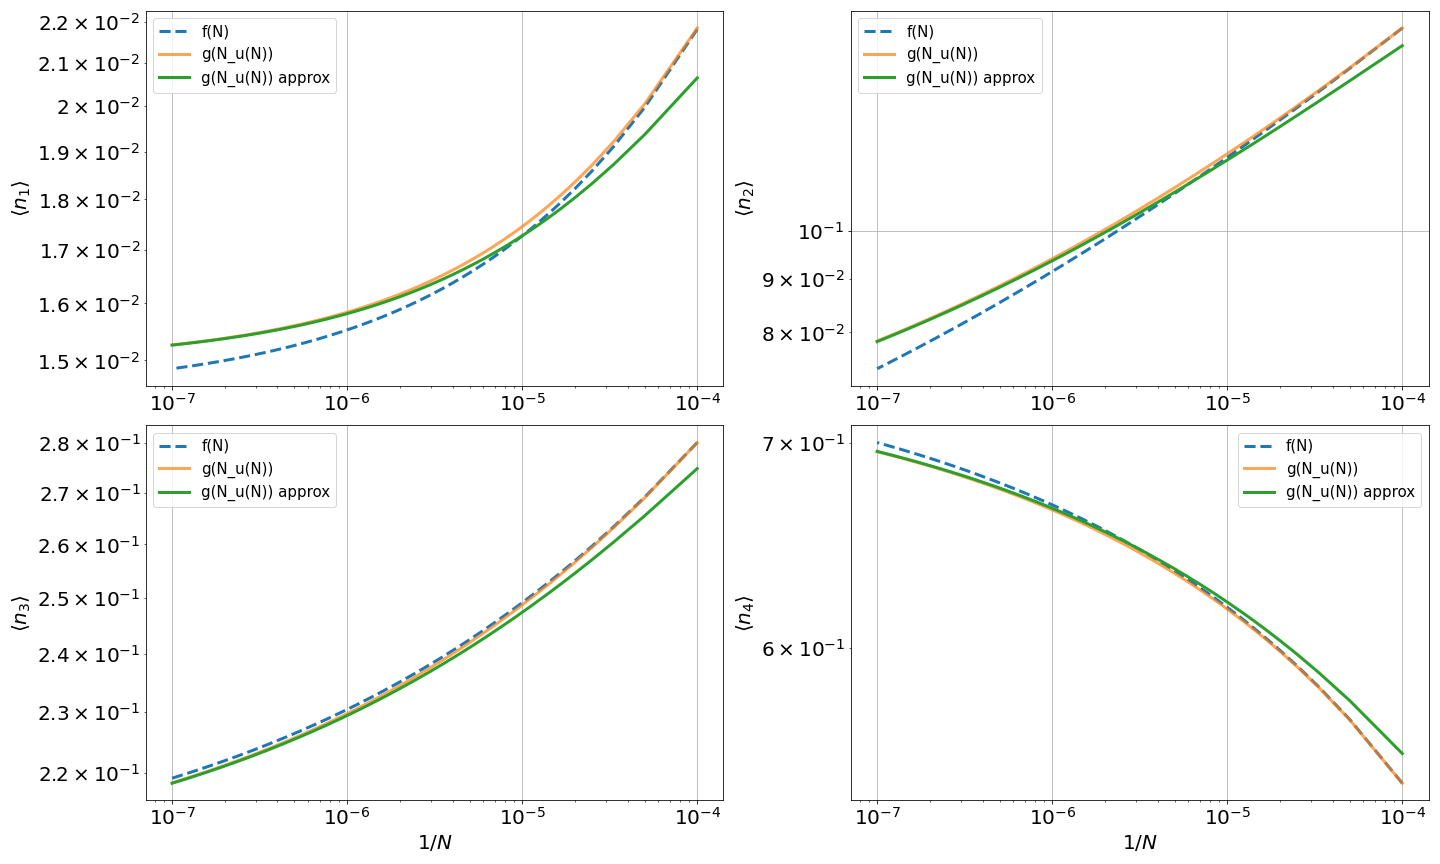
\includegraphics[width=\textwidth]{n_i_fN_vs_gNun_log.png}
\label{fig:ni_fn_vs_gNun_log}
\caption{Доли узлов $n_1-n_4$ в лог-лог масштабе как функции от количества шагов (синий пунктир) \eqref{eq:n_i_log_log}, а так же сложные функции от количества уникальных узлов от количества шагов (оранжевая линия - прямая подстановка функций  \eqref{eq:gi_appprox2} в \eqref{eq:gi_approx1}, зелёная - аппроксимация \eqref{eq:g_n_expect}), по горизонтали - обратное количество шагов блуждания $1/N$. Коэффициеты взяты из таблиц \ref{tab:n_i_log_log} и \ref{tab:n_i_u_log_log}}
\end{figure}
\include{Sections/Bulk_DS_atm}

\chapter{Приложение}
\section{Литературный обзор}

С целью поиска информации о локальном координационном числе (что в случае блужданий может также быть названо числом соседей узла), был проведён обзор литературы, возможно имеющей отношение к рассматриваемым в рамках проекта моделей.

\subsection{Livne, Meirovich: Polymers Adsorbed on a surface}

\subsubsection{Особенности модели блуждания}

В работе \cite{LivneSAW1988} исследуется поведение адсорбирующего случайного блуждания без самопересечений на кубической решётке со следующими особенностями симуляции

\begin{itemize}
    \item Случайное блуждание длины N+1  строится пошагово (N+1 мономеров в цепочке или N шагов), из начала координат (x=0, y=0, z=0) с ограничением на верхнее полупространство (то есть, z >= 0 и плоскость z=0 имеет открытые граничные условия).
    \item Энергия конформации считается как число мономеров, лежащих на поверхности (у которых $z_{i} = 0$), умноженное на константу взаимодействия полимера и поверхности $\epsilon$
    \item Вероятность i-й конформации считается последовательно: вводится новая статсумма, суммирующая для заданного направления текущей недостроенной цепочки всевозможные хвосты остаточной длины (10)\cite{LivneSAW1988}. 
\end{itemize}

\subsubsection{Подробнее о статсумме и методе Сканирования }

В данном подразделе вольным образом объясняется действие статсуммы, созданное методом сканированния. Так как при симуляции строится новое блуждание "c нуля", требуется оценка вероятности как каждого шага (точнее, направления $v_{k}$) так и всего блуждания.

Поэтому для k-го шага вероятность рассчитывается следующим образом:

\begin{enumerate}
    \item Считается статсумма куска будущего блуждания из b ($<= N - k + 1$) шагов, начинающая с направления v на высоте $z_{k-1}$:
    
    \begin{equation}
        Z_{k}(v, b, z_{k-1}, v_{k-1}) = \sum_{j}\exp{(-\epsilon m_{j}(0)/k_{b}T)}
        \label{Z_Lenvi}
    \end{equation}
     
    \item Затем проводится расчёт вероятности выбрать направление v из всех возможных на k-м шаге:
    
    \begin{equation}
        p_{k}(v|b,z_{k-1},v_{k-1}) = Z_{k}(v, b, z_{k-1}, v_{k-1}) / \sum_{v} Z_{k}(v, b, z_{k-1}, v_{k-1})
        \label{p_k_Lenvi}
    \end{equation}
    
    \item Итоговой вероятностью всего построения будет произведение всех вероятностей каждого шага по выбранным направлениям:
    
    \begin{equation}
        P_i(b) = \prod_{k=1}^{N} p_{k}(v_{k}|b,z_{k-1},v_{k-1})
    \end{equation}
\end{enumerate}

\subsubsection{Результаты работы}

Основными итогами работы являлось подтверждение эффективности метода "сканирования" для работы с длинными цепочками в модели адсорбирующего блуждания, определено критическое шкалирование перпердикулярного радиуса инерции (радиуса инерции проекции блуждания на ось z), а также профиля мономерной концентрации $p(z)$ (средняя доля узлов конформации длины N+1 на фиксированной высоте z от поверхности).

Информации о локальном координационном числе в статье найдено не было.

\newpage

\subsection{Madras, Sokal: The Pivot Algorithm}

Работа \cite{madras1988pivot} повествует о работе и эффективности алгоритма Пивота в изучении модели случайного блуждания без самопересечений (СБС).

\subsubsection{Основные принципы алгоритма}

Каждый шаг алгоритма проводит следующие действия над уже сгенерированной цепочкой длины N+1:

\begin{itemize}
    \item Случайно выбирается с равномерным распределением для рассматриваемых узлов $p_{k} = 1/N$ k-й узел цепочки ($0 <= k <= N-1$, хотя начальную точку k=0 на практике не используют)
    \item Последующую половину цепочки ($\omega_{k+1}, \omega_{k+2},\dots,\omega_{N}$ заменяют элементов группы симметрии (проще говоря, отражают, поворачивают или проводят комбинацию этих действий)
    \item В случае, если полученная операцией цепочка осталась без самопересечений, шаг принимается - в противном случае, шаг производится заново
\end{itemize}

В статье так же была доказана эргодичность алгоритма, а так же средние вероятности принятия каждого из возможных преобразований.

Для симуляций в качестве стартовой позиции использовалось два варианта: прямые цепочки ''rods'', при которых проволилось некоторое кол-во шагов до достижения термального равновесия системы (в таком состоянии процесс из следующих состояний цепочки становится близким по расспределению к стационарному стохастическому), или же ''димеризованные цепочки'' , состояние которых уже считается равновесным. Второй метод становится крайне времезатратным при большой длине цепочки, поэтому при N>=2400 чаще применялась термолизация прямых цепочек.

Пристальное внимание в статье было обращено к среднему радиусу инерции $S^{2}_{N}$ и квадрату расстояния между концами $\omega^{2}_{N}$, а так же к оценке метрической экспоненты $\upsilon$, характеризующей обе величины в крит. области модели: 

\begin{align*}
    \la \omega^{2}_{N} \ra &\sim N^{2\upsilon} \\
    \la S^{2}_{N} \ra &\sim N^{2\upsilon} 
\end{align*}

В оценке будущей работы было так же отмечено, что алгоритм Пивота не подходит для расчёта связующей $\mu$ и критической $\gamma$ экспонент (связующую константу так же называют \textit{эффективным координационным числом}), так как алгоритм алгоритм работает лишь в случае канонического ансамбля (при фиксированной длине цепочки) и требуется алгоритм, работающий уже в большом каноническом ансамбле (с цепочками изменяемой длины).

В статье не рассматривалось как таковое ''число соседей узлов''.


\subsection{Спицер, Основные принципы случайного блуждания, глава 3}

Данный подраздел посвящён рассмотрению случая двумерного возвратного случайного блуждания - блуждания, движущемся по состояниям $R$ до достижения одного из элементов $A \subset R$. Под $T$ или $T_A$ мы будем подразумевать момент остановки - минимальное число $1<= k <= \infty$, такое что $x_k \in A$, то есть минимальное время достижение процессом {x_i} состояния из пространства A.

\subsubsection{Основные вероятностные функции}

Здесь будут более тщательно описаны используемые в главе функции вероятностей перехода.

$Q_n(x,y)$ определена на $(R-A) \times (R-A),\ \ n >= 0$ и обозначает вероятность попасть на n-м шаге попасть в $y$ (при $x_0 = x$), не попав за это время в A. Логично, что при остановке $T<n$ вероятность достижения на n-м шаге не существует, т.к. проццесс остановлен.

\begin{equation}
 Q_n(x,y) = P_x[x_n=y; T>n]
\end{equation}

Функция $H^{(n)}_A(x,y)$, наоборот, определяет вероятность n-м шаге остановиться в $y \in A$ (то есть, $y$ является первым состоянием из $A$, в которое попал процесс. В данном случае $H_A$ определено на $R \times A$

\begin{equation}
H^{(n)}_A(x,y) = 
	\begin{cases}
		P_x[x_T=y; T=n], \ \ \ x \in R-A \\
		0, \ \ \ x \in A, n>=1 \\
		\delta(x,y), \ \ \ x \in A, n=0
	\end{cases}
\end{equation}

$H_A(x,y)$ является обобщением предыдущей функции по времени, определяя лишь вероятность остановки процесса, начавшегося в $x$, в $y \in A$ и определена там же как и $H^{(n)}_A(x,y)$.

\begin{equation}
H_A(x,y) = 
	\begin{cases}
		P_x[x_T=y; T < \infty], \ \ \ x \in R-A \\
		\delta(x,y), \ \ \ x \in A
	\end{cases}
\end{equation}

Для случая $x \in R-A$ эту функцию можно определить так же как:

\begin{equation}
H_A(x,y) = \sum^{\infty}_{n=0}H^{(n)}_A(x,y)
\end{equation}

Особым случаем является вероятность $\Pi_A(x,y)$, существование которой обусловлено тем фактом, что время остановки должно быть натуральным числом - строго говоря, процесс может начатся в $x \in A$, пройти по ${x_1, x_2,...x_T-1 \in R-A}$ и остановиться в $y \in A$.

\begin{equation}
\Pi_{A}(x,y) = P_x[x_T=y, T < \infty]
\end{equation}

Последняя функция - $g_A(x,y)$, обобщается по времени $Q_n$:

\begin{equation}
g_A(x,y) = 
	\begin{cases}
		\sum^{\infty}_{n=0}Q_n(x,y), \ \ \ x, y \in R-A \\
		0, otherwise
	\end{cases}
\end{equation}

Из общих понятий нам также понадобится $G(x,y)$ - ожидаемое число попаданий в $y$ при начальной точке $x$:

\begin{equation}
G(x,y) = \sum_{n=0}^{\infty}P_x[x_n=y]
\end{equation}



\section{Программно-техническое приложение}

В данном разделе будут описаны особенности работы с суперкомпьютером НИУ ВШЭ, которые могут быть важными дополнением к основной инструкции пользователя.

\subsection{Применение jit-компиляции при программировании на языке Python}
\label{subsection:njit_problem}

Симуляции случайного блуждания с самопересечениями (для кода см. папку $Random\_Walk$  \cite{web:ProjectMagnetRepos}) были запрограммированны на языке Python с компиляцией с помощью пакета numba метод jit. В качестве окружения была использована стандартная библиотека $Python/Anaconda\_v11.2021$ встроенная в стандартное ПО суперкомпьютера. 

Выполнение первых экспериментов по симуляциям шло крайне медленно - результаты за семь дней можно увидеть на таблице \ref{tab:Ran_Walk_neigh_1}

\begin{table}[h]
    \centering
    \begin{tabular}{|c|c|c|c|c|c|c|}
        \hline
        N & $steps$ & $unique$ & $n_{1}$ & $n_{2}$ & $n_{3}$ & $n_{4}$ \\ \hline
        100 & 7450000 & 0.49(8) & 0.07(3) & 0.33(9) & 0.36(7) & 0.24(9) \\ \hline
        200 & 5684000 & 0.44(7) & 0.05(2) & 0.29(7) & 0.35(5) & 0.30(9) \\ \hline
        500 & 2045000 & 0.39(6) & 0.04(1) & 0.24(5) & 0.34(4) & 0.38(8) \\ \hline
        1000 & 654000 & 0.36(5) & 0.03(1) & 0.22(4) & 0.33(4) & 0.42(7) \\ \hline
        2500 & 132000 & 0.33(4) & 0.027(7) & 0.19(3) & 0.31(3) & 0.48(6)  \\ \hline
        5000 & 37000 & 0.31(4) & 0.024(5) & 0.17(3) & 0.29(3) & 0.51(6) \\ \hline
        10000 & 10000 & 0.29(3) & 0.021(4) & 0.16(2) & 0.28(3) & 0.54(5) \\ \hline
    \end{tabular}
    \caption{Средние доли узлов c 1-4-мя соседями в конформациях модели Random-Walk длин $10^{2}-10^{4}$}
    \label{tab:Ran_Walk_neigh_1}
\end{table}

Для сравнения с другими платформами, в случае длины цепочки $N=10000$, процесс из 10000 шагов на Google Colab занимал не более 7 часов.

\begin{figure}[h]
    \centering
    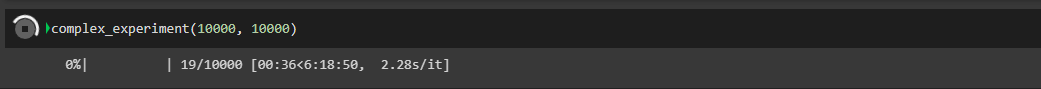
\includegraphics[width=0.95\textwidth]{experiment_time.png}
\end{figure}

Решением проблемы оказалось создание собственного окружения с другими версиями используемых пакетов numpy и numba (полный список так же есть в репозитории с кодом \cite{web:ProjectMagnetRepos}). Новые результаты за 7 дней описаны в продолжении основного раздела.

При обсуждении столь значительного различия во времени выполнениями между окружениями поддержкой было выдвинуто предположение, что окружения отличаются сторонними библиотеками линейной алгебры, используемой пакетом numpy: наиболее распространенными считаются OpenBLAS и Intel MKL. Основным фактором преимущества той или иной библиотеки является именно процессор (Intel или non-Intel). 

В новом окружении пакетом numpy использовалась именно библиотека OpenBLAS, в то время как в Anaconda - Intel MKL. Это следовало из применения в данных окружениях следующего:

\begin{code}
import numpy

print(numpy.show\_config())
\end{code}

Подробнее об определении какая библиотека линейной алгебры используется в пакете numpy можно найти \href{https://shaalltime.medium.com/benchmark-numpy-with-openblas-and-mkl-library-on-amd-ryzen-3950x-cpu-96184f91057f}{здесь}. 


\subsection{Итерации программного комплекса Rand-Walk}

Подраздел посвящён описанию версий программного комплекса для симуляций модели простого случайного блуждания фиксированной длины N на квадратной решётке.
(для кода см. папку $Random\_Walk$  \cite{web:ProjectMagnetRepos})

\begin{enumerate}
\item \textbf{Drunken\_Sailor\_def.py} - базовый алгоритм симуляций, предназначенный для проверки работы основных функций: 
\begin{itemize}
\item experiment - генерация цепочки и подсчёт наблюдаемых (доли узлов с числом соседей 1-4, а так же доля уникальных узлов цепочки)
\item \textit{complex\_experiment} - запись результирующего массива для одной цепочки (experiment) и набора цепочек (шаг - кол-во опытов между анализом данных)
\item \textit{write\_results} - запись текущих результатов (средних наблюдаемых по всем экспериментам) в текстовый файл
\item \textit{save\_distr} - распределение значений наблюдаемых по всем экспериментам
\item \textit{save\_history} - сохранение истории средний значений для анализа сходимости результаотв симуляций
\end{itemize}
Цепочка генерируется как двумерный массив точек, потому наиболее его медленной частью является поиск уникальных узлов цепочки через \textit{np.unique}, не поддерживающий njit-комплиляцию при обработке двумерного массива.
\item \textbf{Drunken\_Sailor.py} - первая версия симуляционного комплекса с jit-компилируемой частью. Алгоритмически не отличается от \textbf{Drunken\_Sailor\_def.py}, но значительно быстрее базовой версии
\item \textbf{Drunken\_Sailor\_v2.py} - оптимизированная версия \textbf{Drunken\_Sailor.py} c расширенной njit-комплиляцией:
\begin{itemize} 
\item \textit{create\_walk} - генерация цепочки как массива поворотов блуждания начиная с начальной точки $(0,0)$, затем - как массив всех точек блуждания
\item \textit{calc\_fractions} - основная функция подсчёта наблюдаемых. Так же модифицирована над подсчёт атмосферы каждого блуждания
\item В \textit{complex\_experiment} добавлено распараллеливание проведение набора экспериментов за шаг между выводом данных, что позволило значительно ускорить работу комплекса.
\item \textit{stats} - подсчёт текущего результата для наблюдаемых долей
\item \textit{atm\_bins} - подсчёт долей блужданий с атмосферой 0-3
\end{itemize}
\end{enumerate}




\bibliographystyle{plain}
\bibliography{bibliography}

\end{document}




